%
% Complete documentation on the extended LaTeX markup used for Insight
% documentation is available in ``Documenting Insight'', which is part
% of the standard documentation for Insight.  It may be found online
% at:
%
%     http://www.itk.org/
%
%
\documentclass{InsightArticle}
\usepackage{graphicx}
\usepackage{listings}	
\usepackage{wrapfig}
\usepackage{amssymb,amsmath}
\usepackage{multirow,booktabs,ctable,array}
\lstnewenvironment{VHDLlisting}[1][]
  {\lstset{
    language=VHDL,
    basicstyle=\footnotesize\ttfamily,
    columns=flexible,
    keepspaces=true,
    keywordstyle=\color{red},
    identifierstyle=\color{green},
    commentstyle=\color{blue},
  }}{}
%%%%%%%%%%%%%%%%%%%%%%%%%%%%%%%%%%%%%%%%%%%%%%%%%%%%%%%%%%%%%%%%%%
%
%  hyperref should be the last package to be loaded.
%
%%%%%%%%%%%%%%%%%%%%%%%%%%%%%%%%%%%%%%%%%%%%%%%%%%%%%%%%%%%%%%%%%%
\usepackage[bookmarks,
bookmarksopen,
backref,
colorlinks,linkcolor={blue},citecolor={blue},urlcolor={blue},
]{hyperref}

\definecolor{customblue}{RGB}{235,241,245}

\lstdefinestyle{mystyle}{%
  backgroundcolor=\color{customblue},
  frame=single,
  framerule=0pt,
  basicstyle=\ttfamily,
  breaklines=true,
  columns=fullflexible
}

\lstnewenvironment{terminalblock}{%
  \lstset{style=mystyle}}{}

\definecolor{listlightgray}{gray}{0.955}

\graphicspath{{./Figures/}}
\newcommand{\R}{\textit{R}}
\newcommand{\fv}{\mbox{\boldmath $f$}}
\newcommand{\Iv}{\mbox{\boldmath $I$}}
\newcommand{\xv}{\mbox{\boldmath $x$}}
\newcommand{\velocity}{\mbox{\boldmath $v$}}
\newcommand{\velocityinv}{\mbox{\boldmath $v$}^{-1}}
\newcommand{\Velocityinv}{\mbox{\boldmath $V$}^{-1}}
\newcommand{\Velocity}{\mbox{\boldmath $V$}}
\newcommand{\welocity}{\mbox{\boldmath $w$}}
\newcommand{\spatialimagegradient}{\mbox{\boldmath $I$}\mbox{$_{x}$}}
\newcommand{\perpspatialimagegradient}{\mbox{\boldmath $I$}\mbox{$^{\perp}_{x}$}}
\newcommand{\temporalimagederivative}{\mbox{$I_t$}}
\newcommand{\finitestrain}{\mbox{\boldmath $\varepsilon^{\ast}$}}
\newcommand{\smallstrain}{\mbox{\boldmath $\varepsilon$}}
\newcommand{\dispgradient}{{\bf \nabla \displace}}
\newcommand{\displace}{{\bf u}} 
\newcommand{\Id}{\text{\bf Id}}
\newcommand{\ode}{{\em O.D.E.}}
\newcommand{\odes}{{\em O.D.E.}s}
\newcommand{\G}{\mathcal{G}}
\newcommand{\J}{\mathcal{J}}
\newcommand{\phiinv}{\phi^{-1}}
\newcommand{\psiinv}{\psi^{-1}}
\newcommand{\dM}{DM}
\newcommand{\DM}{Diffeomorphometry}
\newcommand{\diff}{diffeomorphism}
\newcommand{\Diff}{Diffeomorphism}
\newcommand{\orbit}{\mathcal{O}}
\newcommand{\avg}{\mathcal{A}}
\newcommand{\avgn}{\mathcal{A}_n}
\newcommand{\avgna}{\mathcal{A}^a_{n}}
\newcommand{\nset}{\{ J_i \}_n}
\newcommand{\bari}{\bar{I}}
\newcommand{\bart}{\bar{t}}
\newcommand{\jac}{\mathcal{J}}
\newcommand{\pert}{\mbox{\boldmath $w$}}
\newcommand{\barpert}{\bar{\mbox{\boldmath $w$}}}
\newcommand{\half}{0.5}

\newcommand{\X}{{\bf X}}
\newcommand{\x}{{\bf x}}
\newcommand{\Z}{{\bf Z}}
\newcommand{\z}{{\bf z}}
\newcommand{\p}{{\bf p}}
\newcommand{\Y}{{\bf Y}}
\newcommand{\y}{{\bf y}}
\newcommand{\disp}{{\bf u}}
\newcommand{\ytild}{\tilde{{\bf y}}}
\newcommand{\q}{{\bf q}}
\newcommand{\surf}{\mathcal{S}}
\newcommand{\phij}{\phi_{ij}}
\newcommand{\aphij}{\bar{\phi}_{j}}
\newcommand{\apsij}{\bar{\psi}_{j}}
\newcommand{\aphi}{\bar{\phi}}
\newcommand{\aphiinv}{\bar{\phi}^{-1}}

\newcommand{\domain}{\Omega}
\newcommand{\meanshape}{\bf \bar{x}}
\newcommand{\g}{\mbox{\boldmath $g$}}
\newcommand{\h}{\mbox{\boldmath $h$}}
\newcommand{\yv}{\mbox{\boldmath $y$}}

\newcommand{\group}{Diff}


\newcommand{\evol}{{E_{\text{Vol}}}}
\newcommand{\epair}{{E_{\text{Pair}}}}
\newcommand{\esec}{{E_{S}}}
\newcommand{\inv}{^{-1}}
\newcommand{\vinit}{ \velocity^0_{ij}(\x,\tau=0) }
\newcommand{\avinit}{ \bar{\velocity}^0_{j}(\x,t) }
\newcommand{\avinitz}{ \bar{\velocity}^0_{j}(\x,t_a) }
\newcommand{\gz}{\nabla_{\z}}


%  This is a template for Papers to the Insight Journal. 
%  It is comparable to a technical report format.

% The title should be descriptive enough for people to be able to find
% the relevant document. 
\title{Advanced Normalization Tools (ANTS)}

% 
% NOTE: This is the last number of the "handle" URL that 
% The Insight Journal assigns to your paper as part of the
% submission process. Please replace the number "1338" with
% the actual handle number that you get assigned.
%
%\newcommand{\IJhandlerIDnumber}{}

% Increment the release number whenever significant changes are made.
% The author and/or editor can define 'significant' however they like.
\release{2.x}

% At minimum, give your name and an email address.  You can include a
% snail-mail address if you like.
\author{Brian B. Avants$^1$, Nick Tustison$^2$ and Hans Johnson$^3$}
\authoraddress{University of Pennsylvania$^1$\\University of Virginia$^2$\\University of Iowa$^3$}

\begin{document}
%
% Add hyperlink to the web location and license of the paper.
% The argument of this command is the handler identifier given
% by the Insight Journal to this paper.
% 
%\IJhandlefooter{\IJhandlerIDnumber}


\ifpdf
\else
   %
   % Commands for including Graphics when using latex
   % 
   \DeclareGraphicsExtensions{.eps,.jpg,.gif,.tiff,.bmp,.png}
   \DeclareGraphicsRule{.jpg}{eps}{.jpg.bb}{`convert #1 eps:-}
   \DeclareGraphicsRule{.gif}{eps}{.gif.bb}{`convert #1 eps:-}
   \DeclareGraphicsRule{.tiff}{eps}{.tiff.bb}{`convert #1 eps:-}
   \DeclareGraphicsRule{.bmp}{eps}{.bmp.bb}{`convert #1 eps:-}
   \DeclareGraphicsRule{.png}{eps}{.png.bb}{`convert #1 eps:-}
\fi


\maketitle


\ifhtml
\chapter*{Front Matter\label{front}}
\fi

%Setup listing environment
\definecolor{listcomment}{rgb}{0.0,0.5,0.0}
\definecolor{listkeyword}{rgb}{0.0,0.0,0.5}
\definecolor{listbackground}{gray}{0.965}

\lstset{frame = tb,
        framerule = 0.25pt,
        float,
        fontadjust,
        backgroundcolor={\color{listbackground}},
        basicstyle = {\ttfamily\scriptsize},
        keywordstyle = {\ttfamily\color{listkeyword}\textbf},
        identifierstyle = {\ttfamily},
        commentstyle = {\ttfamily\color{listcomment}\textit},
        stringstyle = {\ttfamily},
        showstringspaces = false,
        showtabs = false,
        numbers = left,
        tabsize = 2,
        language=[ISO]C++,
        floatplacement=!h
        }	

% The abstract should be a paragraph or two long, and describe the
% scope of the document.
\begin{abstract}
\noindent We provide examples and highlights of Advanced Normalization
Tools (ANTs), versions 2.x, that 
address practical problems in real data.  
\end{abstract}

%\IJhandlenote{\IJhandlerIDnumber}

\tableofcontents

\section{Introduction}
This update to ANTs documentation was initiated April 29, 2014.
\textit{This document does not cover all of ANTs functionality --- but
  summarizes the most frequently used components.}
Originally, the ANTs framework provided open-source functionality for deformable
image registration with small or large deformations, as shown in
figure~\ref{fig:chalf}.  Independent evaluation of the 0.0 version of ANTs software, applied to ``control'' data, 
placed the toolkit as a top performer amongst 14
methods \cite{Klein2009}.  Developer evaluation showed stronger differences 
with other methodology in neurodegenerative neuroimaging data, 
where large deformation is required \cite{Avants2008b}. 
ANTs has since grown to include N4 bias
correction \cite{Tustison2010}, additional evaluation of multiple
modalities and organ systems \cite{Tustison2014,Tustison2011,Murphy2011}, univariate or multivariate image segmentation
\cite{Avants2011,Tustison2011a}, tighter integration with the Insight ToolKit \cite{Tustison2013,AvantsITK}, a
well-evaluated cortical thickness pipeline \cite{Tustison2014b} and, more recently,
visualization tools and integration with \R \cite{Tustison2014c}.
ANTs serves as both a core library for further
algorithm development and also as a command-line application-oriented
toolkit.  ANTs also has a permissive software license that allows it
to be employed freely by industry \cite{rosen2004open}.
ANTs enables diffeomorphic normalization with a variety of
transformation models, optimal template construction, multiple types
of diffeomorphisms, multivariate similarity metrics, diffusion tensor
processing and warping, image segmentation with and without priors and
measurement of cortical thickness from probabilistic segmentations.
The normalization tools, alone, provide a near limitless range of
functionality and allow the user to develop customized objective
functions.  Objective functions in ANTs are of the form: $$
\text{Deformation Cost} + \text{Data Terms},$$ and the command
line reflects this balance of two terms.  As mentioned above, the
data term may combine multiple different measures of
similarity that are optimized in parallel, for instance, image similarity 
and landmark terms.  This document seeks to
provide a practical overview of basic functionality and some of the common use cases that
users seek.
Additional information is available online -- see 
\href{http://stnava.github.io/ANTs/}{http://stnava.github.io/ANTs/}.
For compilation details, see:
\href{https://brianavants.wordpress.com/2012/04/13/updated-ants-compile-instructions-april-12-2012/}{https://brianavants.wordpress.com/2012/04/13/updated-ants-compile-instructions-april-12-2012/}
or section~\ref{sec:comp}.
The most important core C${++}$-based ANTs programs are: 
\texttt{antsRegistration, antsApplyTransforms, Atropos} for
segmentation, \texttt{N4BiasFieldCorrection} for
inhomogeneity correction,  \texttt{KellyKapowski} for estimating
thickness, \texttt{ImageMath} image processing utilities
and, finally, \texttt{sccan} for sparse dimensionality reduction.  There
are many other programs which are listed in
\href{https://github.com/stnava/ANTs/tree/master/Examples}{https://github.com/stnava/ANTs/tree/master/Examples}.
The scripts in ANTs wrap the core programs and are in
\href{https://github.com/stnava/ANTs/tree/master/Scripts}{https://github.com/stnava/ANTs/tree/master/Scripts}.
Perhaps the most important are \texttt{antsCorticalThickness.sh}~as a
wrapper of several sub-programs that support our
cortical thickness pipeline \cite{Tustison2014b}, \texttt{antsMultivariateTemplateConstruction2.sh}~for template construction
and \texttt{antsRegistrationSyN.sh}~as a basic interface to a few commonly used registration approaches.
\footnote{This document is a work in progress. Please check for updates with each release.}
\begin{figure}

\includegraphics[width=0.33\textwidth]{Figures/grid1100.pdf} 
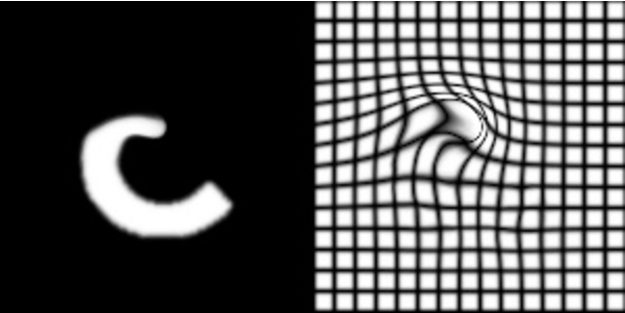
\includegraphics[width=0.33\textwidth]{Figures/grid1110.pdf} 
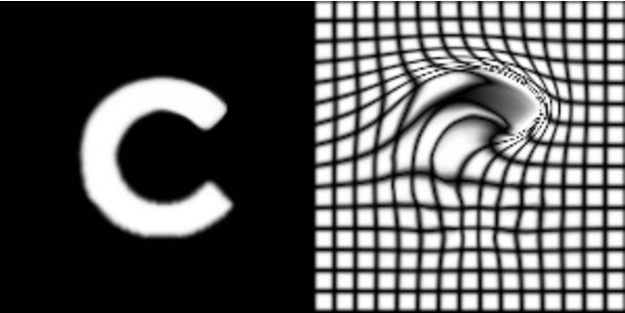
\includegraphics[width=0.33\textwidth]{Figures/grid1119.pdf} 
\itkcaption[ANTs Large Deformation]{The original goal of ANTs was to
  develop public, open source large deformation image registration.
  This is a classic example showing the progress of deforming a half
  C to a full C along a geodesic diffeomorphism.  The deforming 
  grid accompanies each deformed image.  See
  \href{http://stnava.github.io/C/}{http://stnava.github.io/C/} for
  example data and code.}
\vspace{-0.1in}
\label{fig:chalf}
\end{figure}
\subsection{Structure of this document and its examples}
This document is generated with \LaTeX ~and is version controlled at
\href{https://github.com/stnava/ANTsDoc}{https://github.com/stnava/ANTsDoc}.
The examples, here, have data and example scripts stored at dedicated
github repositories, to which we will refer.  Other (simpler) examples will use
data and scripts that are stored in the ANTsDoc git repository.  These
scripts are (loosely speaking) tested and should serve as reproducible
examples for the reader to try.  All data and code is available via
ANTs-related repositories.  The \texttt{compile} script builds both
latex and tests the example scripts.

\subsection{Example 1: Quick SyN}
If you want a decent, fast registration you might run something like this:
\lstinputlisting[style=mystyle,linerange={3-1000}]{examplesandtests/Ex1.sh}
The variable \texttt{\$op} represents the output prefix for the
filename.  This will be the case in many of the following examples.
The \texttt{-d} option denotes image dimensionality, \texttt{-f} option denotes the ``fixed'' image and the \texttt{-m} option
denotes the ``moving'' image.  The moving image will be deformed to
match the fixed image.  The inverse of these maps deform the fixed to
the moving image.  Output is determined by \texttt{-o} where the output
will be named with prefix$=$outputEx1.sh (the word output concatenated
with the name of the Example 1 script) and include a
prefix0GenericAffine.mat (the low-dimensional affine transform which
may be inverted numerically), the prefix1Warp.nii.gz (the
diffeomorphic transformation pulling the affine transformed moving
image toward the fixed image), and the prefix1InverseWarp.nii.gz (the inverse
diffeomorphic transformation pulling the fixed image toward the affine transformed moving
image).
The caveats for this ``canned'' approach include:  1. registration
performance can always be improved by using prior knowledge
\cite{Wolpert1997}; 2. there are many assumptions about the data
embedded in the above call and they may not be appropriate for
whatever problem is at hand; 3. you must have some facility with the command line
to run a shell script.  It is, in general, better to understand a
little bit about image registration rather than running methods
blindly.   To aid readers in this, we have two options: 1. github
issues
\href{https://github.com/stnava/ANTs/issues}{https://github.com/stnava/ANTs/issues};
2.  sourceforge discussion or help sites
\href{http://sourceforge.net/p/advants/discussion/}{http://sourceforge.net/p/advants/discussion/}.
Feel free to use either to ask clarifying questions.  We note that many
issues have been discussed previously and you might find answers by
searching the archives.

\subsection{The \texttt{antsRegistration} executable}
The \texttt{antsRegistration} program itself is the central program encapsulating
normalization/registration functionality.  Its main output is an
affine transform file and a deformation field, potentially with
inverse.  Options allow the user to navigate the similarity
and transformations that are available.  \texttt{antsRegistration} allows multiple
similarity and optimization criteria as options.  The program is
wrapped in \texttt{antsRegistrationSyN.sh} for normalization with ``out of the box''
parameters and in \texttt{antsMultivariateTemplateConstruction2.sh} for 
computationally distributed optimal (multivariate) template construction.

\subsubsection{Initializing \texttt{antsRegistration}}
You can use the  \texttt{-r} option in \texttt{antsRegistration} to
initialize a registration with an ITK .mat format transformation matrix, with a
deformable mapping or with a center of mass alignment.  See the
scripts for examples.  The output transformation will include the
initial transformation. \textcolor{red}{FIXME need to check this}.


\subsection{The \texttt{antsApplyTransforms} executable}
The \texttt{antsApplyTransforms} program applies ANTs mappings to
images including scalars, tensors, time-series and vector images.  
It also composes transforms together and is able to compute
inverses of low-dimensional (affine, rigid) maps.  
\texttt{antsApplyTransformsToPoints} similarly works on point sets (see
\href{http://stnava.github.io/chicken/}{http://stnava.github.io/chicken/} for details).  One may apply an 
arbitrarily long series of transformations through these programs.  Thus, they enable one 
to compose a series of affine and deformable mappings and/or their
inverses.  One may therefore avoid repeated interpolations of a single
image.  Several different
interpolation options are available and multiple image types may be
transformed including:   tensors, vectors, timeseries and
$d$-dimensional scalar images where $d=2, 3, 4$.

\subsection{Using \texttt{antsApplyTransforms} or \texttt{antsApplyTransformsToPoints}}
For example: to apply the transform to the moving image and the
inverse to the fixed image:
\lstinputlisting[style=mystyle,linerange={3-5}]{examplesandtests/Ex2.sh}
The numbers of the transformations (here, 0 and 1 because there is
only a deformation and affine mapping) relate to the order in which
the transforms are computed, during optimization, and also the order
in which they should be applied.  There is reasonably complete
discussion of this framework in \cite{AvantsITK}.

The usage of \texttt{antsApplyTransformsToPoints} is nearly identical.
\textit{However}, it is critical to recognize that transforms that are
one-to-one and onto in image space may not be in point space.
Therefore, points are transformed by the inverses of the
transformation that is applied to images.   This is discussed in
several places in the image registration literature but we first
discussed this in \cite{Avants2006d}.

\subsection{The \texttt{antsMotionCorr} executable }
Performs motion correction of time-series data.  Control parameters
are similar to \texttt{antsRegistration}.  See the example
\href{http://stnava.github.io/fMRIANTs/}{http://stnava.github.io/fMRIANTs/}.
This example also shows how to run basic CompCor on fmri data.  Our
minimal fMRI pipeline involves running \texttt{antsMotionCorr} and
\texttt{CompCorr} to factor out nuisance variables.  More complex
approaches require \textit{ANTsR}.

\subsection{I/O data formats in ANTs}
ANTs supports 2D, 3D and, in some cases, 4D images. 
Since ANTs is implemented in concert with the Insight ToolKit (ITK) \href{http://www.itk.org/}{http://www.itk.org/}, 
it is able to read and write the popular data formats supported
through ITK.  ANTs also uses the ITK view of world-coordinates which
can be confusing, at times, when one is mixing software.  There is
much discussion of this on the web and in ANTs discussion
sites/issues.  Whatever is relevant for ITK
world coordinates is relevant to ANTs as these two software systems
agree, in their entirety, about what the voxel to physical space
coordinate mapping should be. 
There are four basic types of data for ANTs.
\subsubsection{Image volumes}
ANTs supports 2D, 3D, 4D images, including
\begin{itemize}
\item Nifti (.nii, .nii.gz)
\item Analyze (.hdr + .img / .img.gz)
\item MetaImage (.mha)
\item Other formats through itk::ImageFileWriter / itk::ImageFileWriter such as jpg, tiff, etc.  See ITK documentation. 
\end{itemize}
\subsubsection{Affine transformation file}
ANTs uses the itk::TransformFileReader / itk::TransformFileWriter to handle affine transformation files. 
These are Matlab like .mat files recording the matrix and offset for
the low-dimensional transforms: translation, rigid, affine.
The ordering of a matrix transformations parameters breaks down like
this: if parameters are,  $ a~b~c~d~e~f~g~h~i~j~k~l $ , with origin
(or FixedParameters), $ M~N~O $, then the matrix components (rotation,
scaling, shearing all composed together) are:

$ \begin{matrix}
a & b & c \\
d & e & f  \\
g & h & i \\ 
\end{matrix} $

followed by  $~j~k~l~$ (the translation) where $L~M~N$  is the center
of rotation.

\subsubsection{Deformation field file}
ANTs writes the deformation field using image formats that can store
multi-dimensional pixels, usually a nifti-image.  The values of each
pixel are the displacements in physical space.   So, $y=u(x)+x$ where
$u(x)$ is the displacement at $x$.

\subsubsection{Labeled point sets---\textit{Currently not supported by
  antsRegistration, only by old ANTS}}
There are three formats supported
\begin{itemize}
\item  Labeled point sets are saved as an image volume with the intensity = 1,2,3 for label = 1,2,3. For example, 
figure~\ref{fig:frown} shows 2D images representing a 3-class labeled point set. 
\item CSV Format. In this simple format, the point sets are saved as a
  text csv file.  See the chicken example for details \href{http://stnava.github.io/chicken/}{http://stnava.github.io/chicken/}.
\end{itemize}

\subsection{The \texttt{ImageMath} executable} This is a multi-purpose program
that has the following syntax:  \texttt{ImageMath ImageDimension
outputfilename   Operation  InputFileName  parameters} ...  Most basic
scalar image operations -- and some tensor operations -- may be
performed with this program.  Some operations output text files, some
output images and some output only to the terminal.   \texttt{ImageMath} allows
one to multiply images together (m), to negate images (Neg), to take
an image to a power (pow), to test the invertibility of
transformations (InvId), to compute the fractional anisotropy of an
image (TensorFA) and to compute the gradient or laplacian of an image
(Gradient, Laplacian).   Many other operations are available.  Like
all other ANTs programs, one may call \texttt{ImageMath} from the
command line to see all of its options.   \texttt{ImageMath} is used
heavily in ANTs scripts.  
\lstinputlisting[style=mystyle,linerange={3-1000}]{examplesandtests/ExAniDiff.sh}
Above, ImageMath's anisotropic diffusion.
\begin{figure}
\includegraphics[width=0.3\textwidth]{Figures/outputExAniDiffad1.jpg} 
\includegraphics[width=0.3\textwidth]{Figures/outputExAniDiffad2.jpg} 
\includegraphics[width=0.3\textwidth]{Figures/outputExAniDiffad3.jpg} 
\itkcaption[AniDiff]{The original image with 2 degrees of anisotropic diffusion.}
\vspace{-0.1in}
\label{fig:cmd}
\end{figure}


\subsection{ANTs/Scripts} 
The ANTS/Scripts directory contains (hopefully) user-friendly
wrappings of ANTs tools that enable higher-level error checking and
combinations of basic ANTs functions.  These scripts are called as
\texttt{bash}  \texttt{antsscriptname.sh}  and provide usage when called
from the command line.  For instance, try \texttt{bash}  \texttt{antsRegistrationSyN.sh}.
Additionally, if you run ants in tcsh shells, you will need to call it
as follows (using \texttt{antsRegistration} as an example):
\begin{verbatim}
antsRegistration -d 2 -m CC\[r16slice.nii,r64slice.nii,1,2\] ...
\end{verbatim}
instead of
\begin{verbatim}
antsRegistration -d 2 -m CC[r16slice.nii,r64slice.nii,1,2 ] ...
\end{verbatim}
because tcsh does no interpret the brackets as intended.  Using the
bash shell script interface also avoids this.  The key change involves using the slash to force tcsh to 
interpet the bracket literally. 
\newpage
\section{Image registration with ANTs}
\begin{wrapfigure}{r}{0.5\textwidth}
\framebox[0.5\textwidth]{
\begin{minipage}[t]{0.45\textwidth}
{\bf Quick Start:} {\color{blue}call \texttt{antsRegistrationSyNQuick.sh}  (after copying the contents of ANTs/Scripts/ to your bin directory)
  to get usage and apply a normalization to some of your existing
  data.  It is instructional to read the script, modify some of the
  parameters and re-run to witness the effect of your changes -- image
  registration is an art as well as science.  Many other ``ready to
  go'' scripts are available in ANTS/Scripts. Often, the user must set
  his/her ANTSPATH environment variable  -- which points to the
  location of ANTs binaries -- within these scripts or export the
  ANTSPATH variable into the user or script environment.  Note: All ANTs programs provide usage when called from the command line.  Most require the image dimension to be specified as the first parameter.  E.g. 
  \texttt{ImageMath} ImageDimension where ImageDimension is 2, 3, 4.}
\end{minipage}}
\end{wrapfigure}
There are two general applications of image registration. The first
application is transforming labeled data from a template image space
into an individual space. This strategy is important when appearance
alone is not enough to locate a structure as, for example, in the case
of hippocampus segmentation. The template provides a prediction of the
hippocampus-amygdala boundary.  Mapping multiple templates to an
individual (multi-template labeling) can further improve accuracy \cite{Wang2011,Avants2011a}.
The second application operates in the ``inverse'' direction of the first: instead of mapping template to individual, we map individual(s) to the template. Voxel-based population studies of either functional or structural variables depend on mapping to a template space. The common coordinate system enables a statistical evaluation of the likelihood of consistent activation across a group or, in other contexts, the differences in anatomy between two groups. 

The ANTs toolkit enables both types of mapping. The main challenge in image and brain mapping is defining the way in which images/anatomy are compared. There are two components to the comparison.
The shape transformation space defines the range of shape variation that will be allowed in the optimization.
The appearance similarity space defines the statistical assumptions that determine when one image is considered to appear similar to another. 

These two components interact in a weighted optimization within a multiple resolution gradient descent framework. Each component may use either ``strict" or ``flexible" assumptions about the shape or appearance similarity. The selection of these models should be done in a principled way that fits the problem at hand. No single choice is appropriate for all scenarios (see the ``no free lunch" theorem). 

Thus, ANTs enables many operating points from both the transformation and appearance domains such that users may make choices appropriate for their problems. The ANTs command-line syntax, shown in figure~\ref{fig:cmd}, reflects these operating points and the various components that interact in the optimization.
\begin{figure}
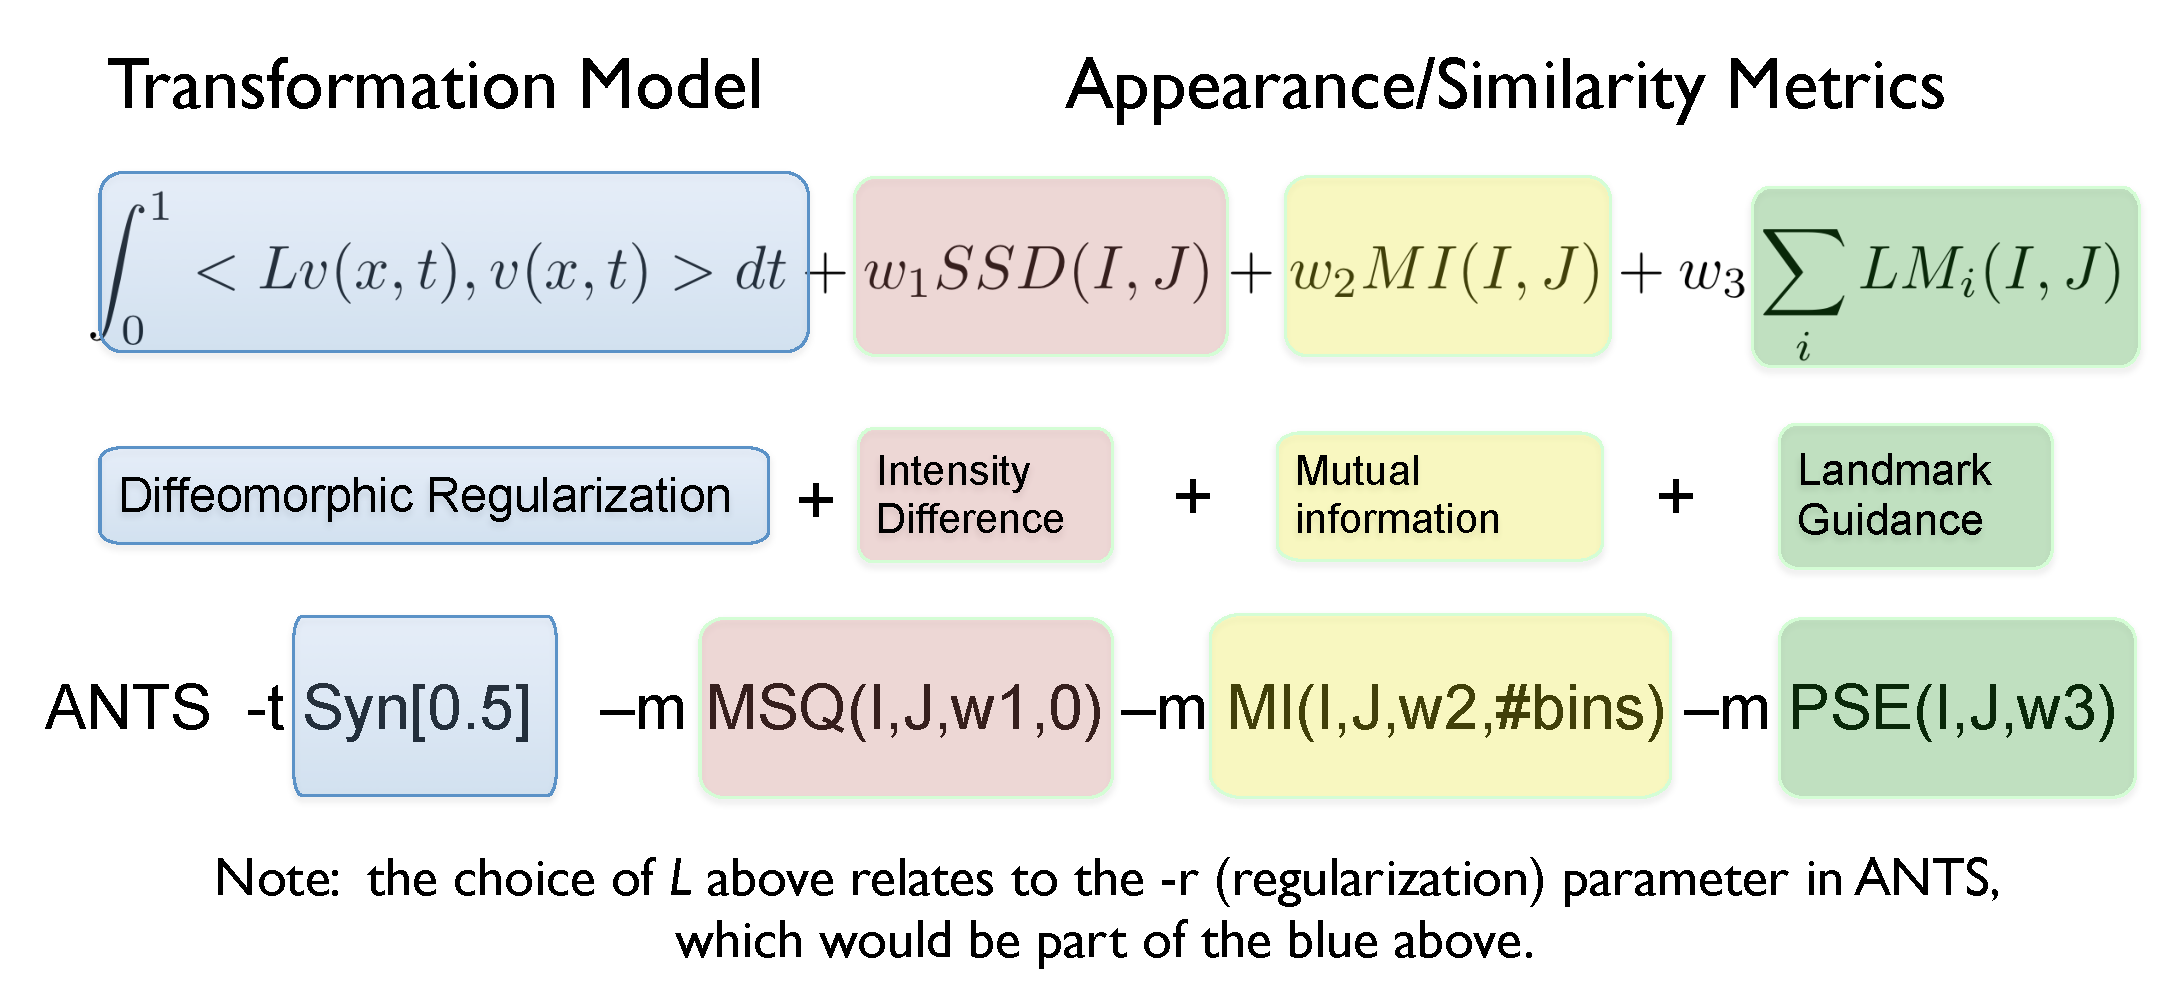
\includegraphics[width=0.9\textwidth]{Figures/ANTSSyntax.pdf} 
\itkcaption[ANTs Command Line]{The relationship between the variational 
form that defines the optimization goals and the ANTs command line.  The 
SyN option implements the method in \cite{Avants2008b} and evaluated in 
\cite{Klein2009}.  The newer version of the ants registration
executable is called \texttt{antsRegistration} and uses a similar
command line that is connected to the variational objective function.}
\vspace{-0.1in}
\label{fig:cmd}
\end{figure}
ANTs may be used to navigate the transformation and similarity metric space. 

\subsection{World coordinates: Use your header!} ANTs uses the direction/orientation, spacing
and origin in its definitions of the mapping between images.  That is,
ANTs uses the ITK standard defintions of an image space.  So, the
image orientation, direction matrix, origin and spacing are important!
If in doubt about, for example, which side is viewed as left or right
by ANTs, then take a look at ITK-SNAP \href{http://www.itksnap.org}{http://www.itksnap.org} and label an image's known left
side.  Then apply an ANTs or ITK mapping to the image to see how the
data is transformed.  \textit{ITK and ANTs do not use the s-form that
  may be stored in some Nifti images.}

DICOM, ITK and ANTs use LPS coordinate systems.  
In contrast, the nifti coordinate system is RPI.  
These coordinate system differences create much confusion
especially when switching between software.  Very
few medical imaging software systems are internally consistent w.r.t. the
treatment of world coordinates across file formats.
However, ANTs and ITK tools will be consistent.  ITK-SNAP will be
mostly consistent with ANTs and ITK although it allows coordinates to
be transformed and, in that case, all bets are off.  As above, if you have a concern, please
perform a straightforward experiment to test your concerns.  Keep in
mind that viewing images with software that does not conform to ITK
world coordinates will make the images ``look wrong'' with respect to
image orientation.  This caveat may include NiPy, FSL, SPM etcetera.

\subsection{ANTs transformation models}
The ANTs toolkit provides a hierarchy of transformations with
adjustable levels of complexity, regularization, degrees of freedom
and behavior as optimizers.  The simplest transformation model is the
translation, followed by the rigid and/or affine transform.  The most complex -- and most flexible
-- is a symmetric diffeomorphic transformation based on optimizing and
integrating a time-varying velocity field.  Computation time also
increases with transformation model complexity, but most normalization
needs may be met with under an hour of computation.  
We provide an overview of some of the ANTs models below and 
try to communicate intuition on what one gains/loses with each choice.  
An overview of available models and similarity terms is in Table~\ref{table:chart}.
\begin{table*}
  \centering
    \begin{tabular}{c c c c}
    {\bf Category} & {\bf Transformation, $\phi$} & {\bf Similarity Measures} & {\bf Brief Description} \\
    \toprule     
    \multirow{2}*{\bf Linear}
           & Rigid$^\dagger$ & MI, MeanSquares, GC & Rigid registration. \\
       {} & Similarity$^\dagger$ & MI, MeanSquares, GC & Rotation +
       uniform scaling. \\
       {} & Affine$^\dagger$ & MI, MeanSquares, GC & Affine registration. \\
       \cmidrule(l){2-4}
    \multirow{2}*{\bf Elastic}
           & GaussianDisplacementField & CC, MI, MeanSquares, Demons & Demons-like algorithm. \\
       {} & BSplineDisplacementField & CC, MI, MeanSquares, Demons  & FFD variant. \\
       \cmidrule(l){2-4}
    \multirow{2}*{\bf Diffeo.}
           & Exponential$^\dagger$ &  CC, MI, MeanSquares, Demons& $~\min~\velocity(\x)$ \\
       {} & SyN$^\dagger$ &  CC, MI, MeanSquares, Demons  & ~locally in time~$\min~\velocity(\x,t)$\\
       {} & BSplineSyN$^\dagger$ &  CC, MI, MeanSquares, Demons  & ~locally in time~$\min~\velocity(\x,t)$\\
       {} & TimeVaryingVelocityField$^\dagger$ &  CC, MI, MeanSquares, Demons  &  $~\min~\velocity(\x,t)$ over all time \\
    \bottomrule
    \end{tabular}
  \caption{Transformations and a subset of the similarity metrics
    available in ANTs.  Similarity metric acronyms:  CC = neighborhood
    cross correlation (the preferred metric), MeanSquares = mean
    squared difference, MI = mutual information, PSE = point-set
    expectation (to be added soon-ish \textcolor{red}{FIXME}) \cite{Pluta2008}.  ANTs also provides the inverse of those transformations denoted by the `$\dagger$' symbol.  The brief descriptions of the diffeomorphic algorithms contrast the way in which the velocity field is optimized and used to parameterize $\phi$, the mapping.  All 
ANTs Diff algorithms generate $\phi(\x,t)$ over $t \in [ 0, 1]$ through gradient descent.}
  \label{table:chart}
\end{table*}    
\vspace{0in}

\paragraph{General Parameters:} ANTs registration options include control of iterations (and,
optionally, convergence criterion) via
\texttt{-c 5000x5000x5000} which specifies that the affine registration
uses a 3 level image pyramid with each level 5000 iterations at
most.  Multi-resolution options include \texttt{-s} for smoothing and
\texttt{-f} for ``shrink factors'' i.e. downsampling rates (e.g. 8
means 1/8$^{th}$ resolution).  
\texttt{MI[fixed,moving,1,32,Regular,0.1]} means to use Mutual
Information as similarity metric with 32 bins and regularly spaced
samples of 10\% of the image; lower sampling rates increases speed and
is useful in low-dimensional registration.  \texttt{MI[fixed,moving,1,32]} means to use Mutual
Information as similarity metric with 32 bins and dense sampling of
the image and would be typically used in deformable registration. See \texttt{antsRegistration --help}
for more information. 

\subsubsection{Affine and rigid
  registration---\textcolor{red}{FIXME---this section and figures}}


\begin{figure}
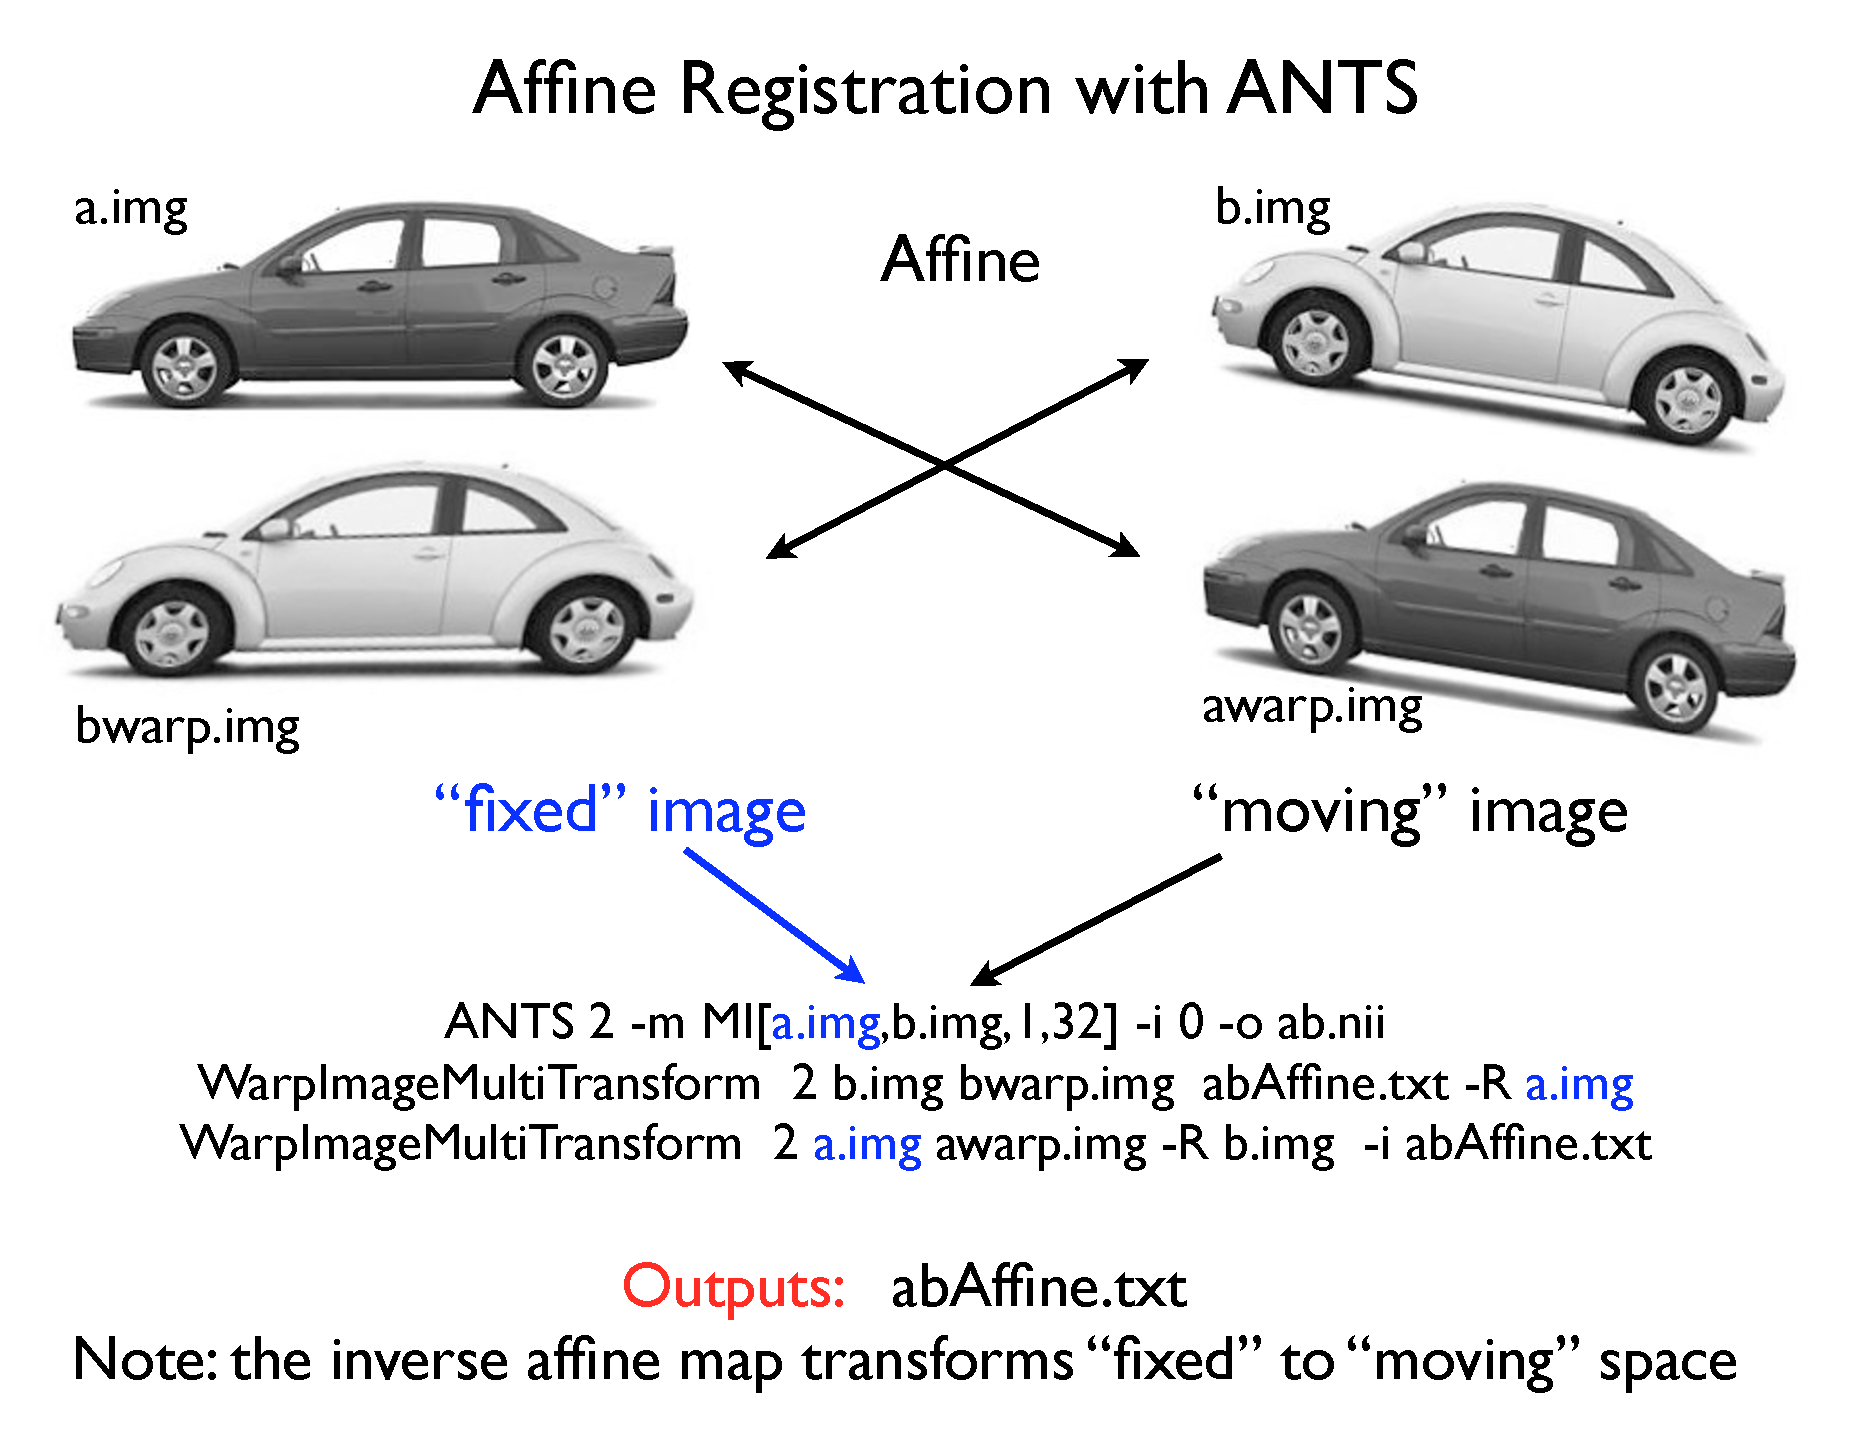
\includegraphics[width=0.9\textwidth]{./Figures/ANTSanatomy.pdf} 
\itkcaption[ANTs Introduction]{The anatomy of an ANTs optimization and application of the resulting warping.}
\vspace{-0.1in}
\label{fig:aff}
\end{figure}
The ANTs affine mapping syntax is shown in the affine mapping
figure~\ref{fig:aff}. 

Affine mapping may become nontrivial when the region of interest 
occupies only a small portion of the image data.  In such cases, 
ANTs enables the user to define a mask to focus the optimization 
effort on the region of interest.  
Example code for (affine) registration with a mask: 
\href{http://stnava.github.io/BasicBrainMapping/}{http://stnava.github.io/BasicBrainMapping/}.
The difference between this command 
and a regular ANTs call is the \verb"-x" option, which specifies the mask, defined in the 
template space.   The mask option also affects the deformable
optimization. 



\noindent{\bf Rigid Registration: }  ANTs will also perform rigid registration.  For example,  
\lstinputlisting[style=mystyle,linerange={3-1000}]{examplesandtests/Ex3.sh}
The jacobian of the resulting affine mapping should be unity.  Compare
the \texttt{antsRegistrationSyNQuick.sh} and
\texttt{antsRegistrationSyN.sh} scripts to see how one might improve
or modify registration parameters for different problems.

\subsubsection{Deformable registration}
Affine mapping is adequate when the
difference between images involves only rotation, scaling or shearing.
Other data requires more deformable mappings to capture shape
differences and find a good alignment of image features.
Figure~\ref{fig:antshier} shows how deformable mapping may improve the
correspondence of the deformed beetle to the ford image.
\begin{figure}
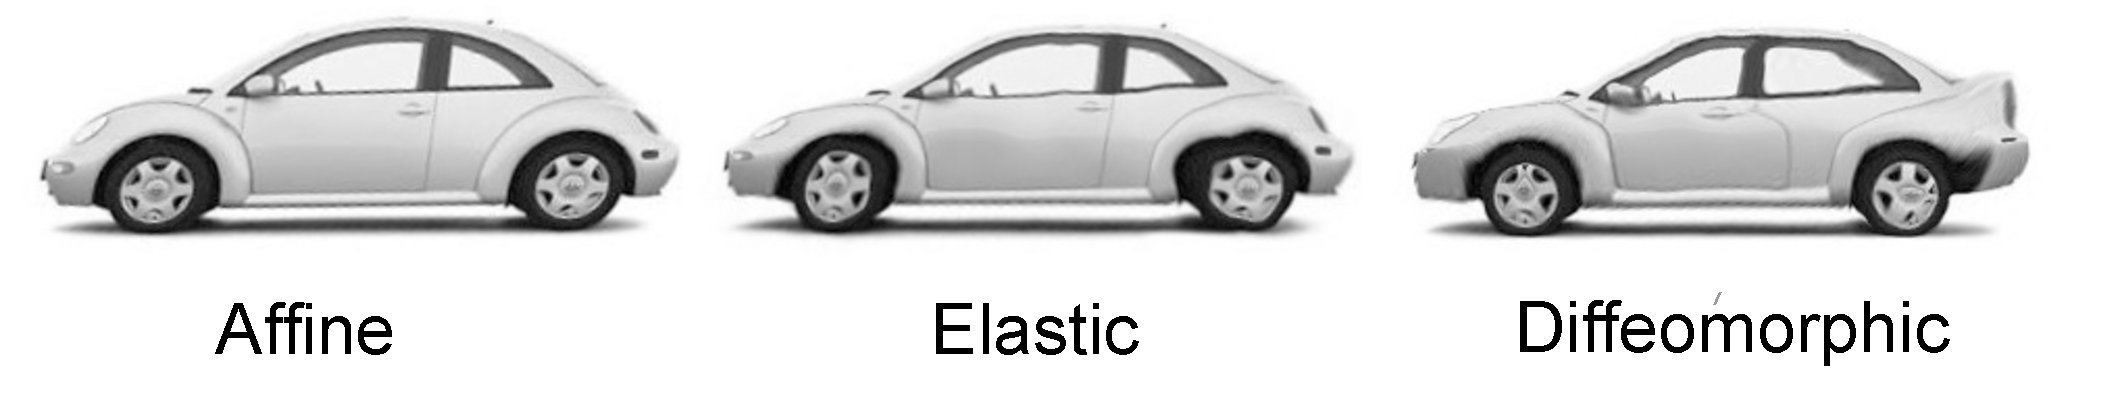
\includegraphics[width=0.9\textwidth]{./Figures/ANTSElastToDiff.pdf} 
\itkcaption[ANTs Transformation Examples]{This example shows the degree to which the beetle (b.img) may be deformed to the ford (a.img) under different transformation models.  Left to right increases the degrees of freedom in the mapping and thus the registration accuracy.}
\vspace{-0.1in}
\label{fig:antshier}
\end{figure}
Most ANTs-based applications use symmetric diffeomorphic normalization.  However, 
ANTs also enables a simpler parameterization of a deformable mapping via a regularized 
vector space.  We term these types of transformations as ``elastic''.  The original Demons algorithm 
provides a classic example of using a regularized vector space for nonlinear registration.  
Caveats are that a regularized vector space may not preserve the underlying topology 
and may also prove too inflexible to capture the shape changes one is after.  Both of these 
shortcomings motivate the use of diffeomorphisms. 

\noindent{\bf Elastic/Vector Space Transformations.} If we assume no affine transformation, then 
an elastic transformation involves computing a mapping from image $I(\x)$ to image $J(\x)$ 
through a deformation field $\disp( \x )$.  
\begin{figure}
\center 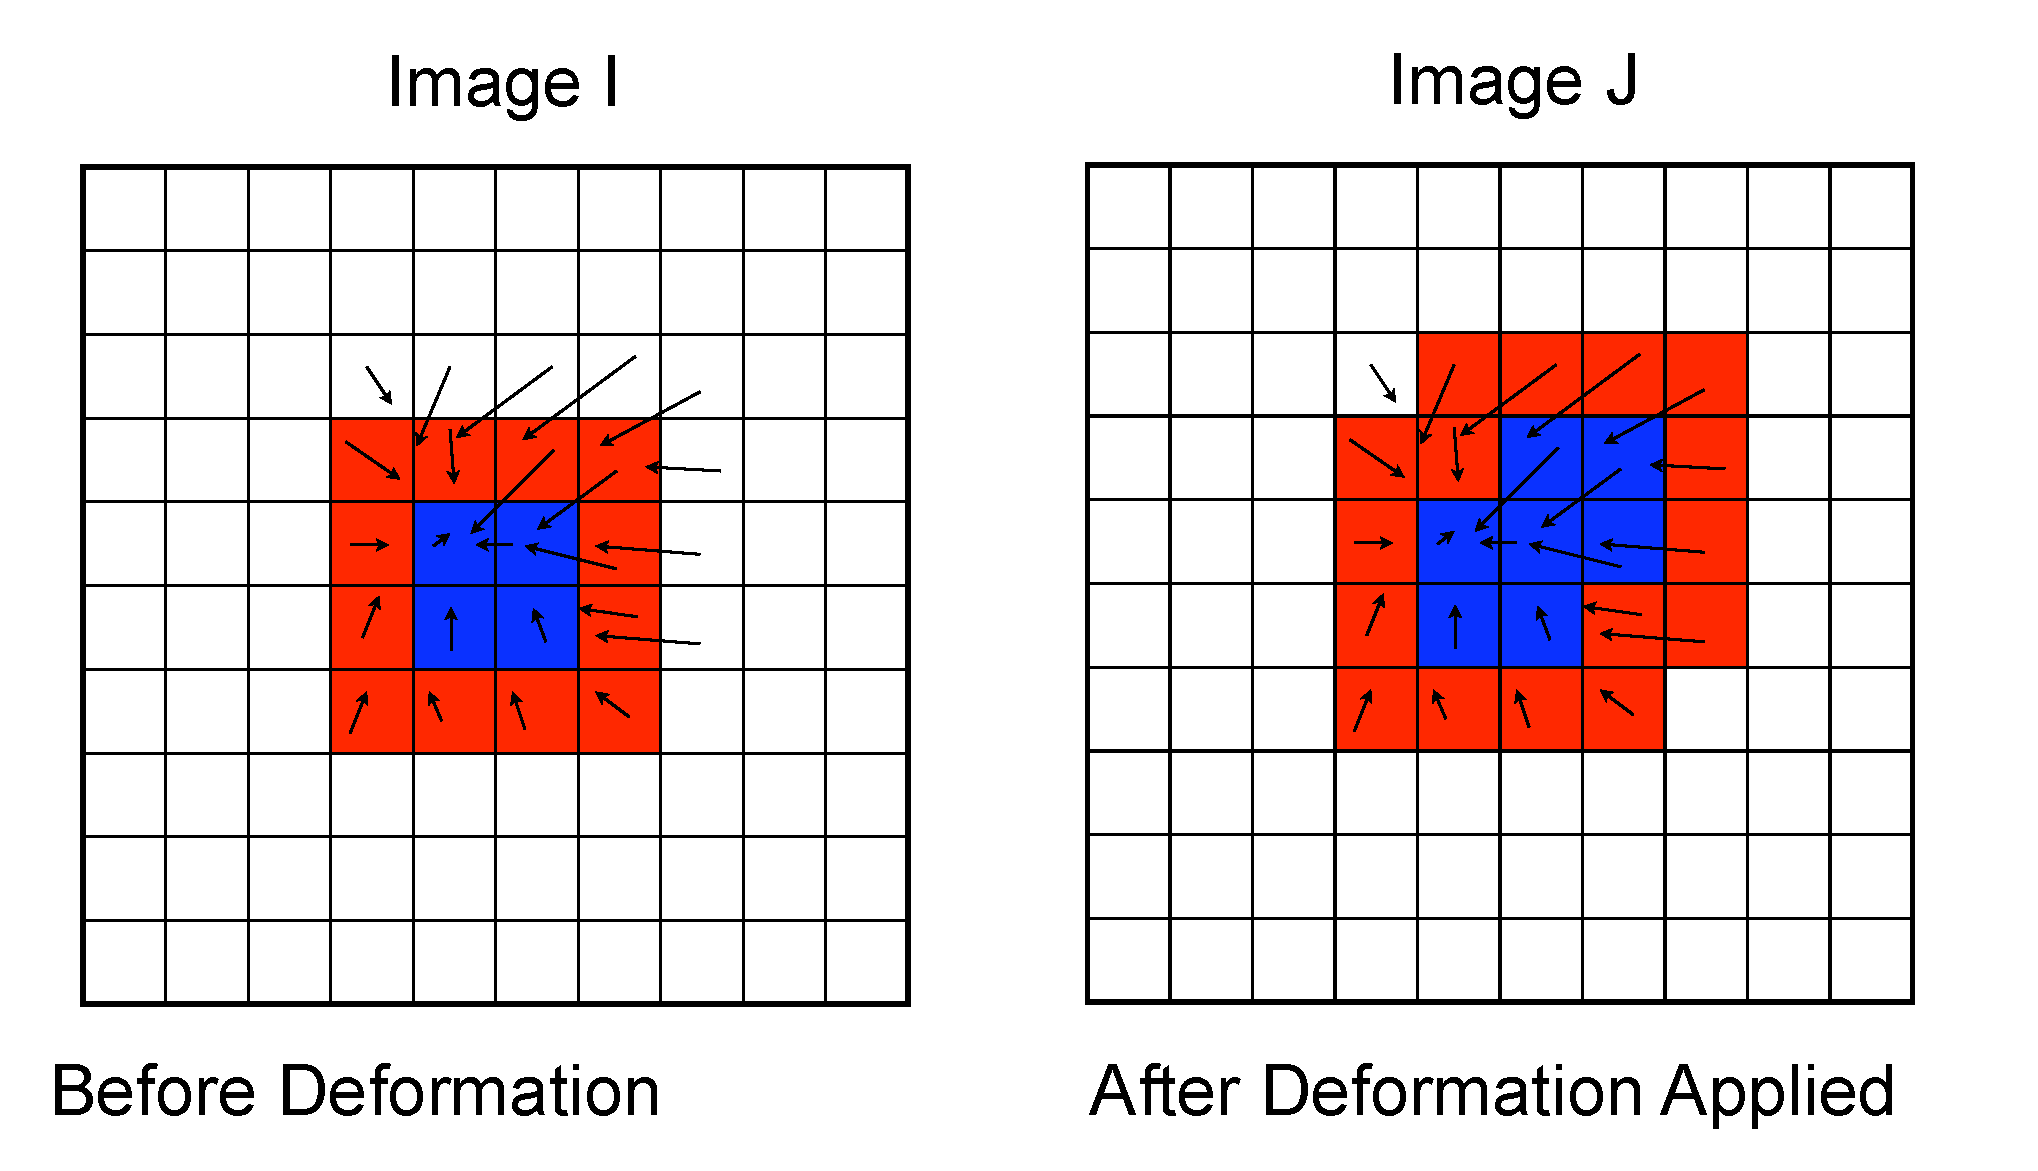
\includegraphics[width=0.75\textwidth]{./Figures/PullBack.pdf} 
\itkcaption[ANTs Deformation]{A deformation in a digital domain.}
\label{fig:pull}
\end{figure}  
The deformation is defined in the physical space of the image 
and dictates the positional difference between corresponding features in the two images.  
Thus, if a feature defined at $I(\x)$ matches a feature in $J$ at position $\y$ then the deformation 
field at $\x$ should give $\disp ( \x )=\y-\x$.   
Such a deformation field may be applied to deform 
image $J$ into image $I$ by composing the mapping $J_{deformed}(\x)=J(\x+\disp(\x))$.  
In a perfect world, then $I(\x)=J_{deformed}(\x)$, though this is rarely the case.  Figure~\ref{fig:pull} 
visualizes the deformation of an image under this standard model. 
Gradient descent optimization of an elastic mapping may be summarized (crudely) as: 
\begin{align}
\text{Compute the similarity gradient:   }  \nabla E = \partial_{\disp} \Pi(I,J(\x+\disp(\x))). \nonumber \\
\text{Update the deformation field:  }  \disp(\x) \leftarrow \disp(\x)+\delta \nabla E. \nonumber \\ 
\text{Regularize the deformation field:  }  \disp(\x) \leftarrow G_\sigma \star \disp(\x),
\end{align}
where $\Pi$ is the similarity, $\delta$ is a gradient step length and $G_\sigma$ is a gaussian smoother.
This optimization is captured in the following ANTs command (\textcolor{red}{FIXME})
\lstinputlisting[style=mystyle,linerange={3-1000}]{examplesandtests/Ex4.sh}
Here, we use the CC metric (a cross-correlation implementation) with
window radius 4, weight 1 and gradient step length 1.5.  The
optimization will be performed over three resolutions with a maximum
of 30 iterations at the coarsest level, 20 at the next coarsest and 10
at the full resolution.  We use a Gaussian regularizer with a sigma of
3 that operates only on the deformation field and not on the similarity gradient, as 
0 is passed as the first parameter to \texttt{GaussianDisplacementField} .  One may see the
correspondence, yet again, between the ANTs call and the optimization
scheme.  The optimization will stop when either the energy cannot be 
smoothly minimized or the maximum number of iterations is reached. 
BSpline regularization is also available in ANTs -- see the DMFFD 
section below.  

\noindent{\bf Warping and Invertibility.}  ANTs uses physical space to
define mappings. The origin etc is in the coordinates of the world in
which the picture (e.g. MRI) was taken. Then, warping between physical
coordinates is relatively easy. Differences in bounding boxes etc
present no problem -- assuming you avoid inconsistent headers
i.e. origins, directions, data orientation. One may use PrintHeader to
check the data and run simple, fast tests (few iterations) to perform
sanity checks before running through loads of data.
An ANTs deformation consists of
a standard naming prefix plus a standard naming extension. We usually 
assume nii but other file types may be used. The value of a voxel of a deformation/warp component
image is the physical space displacement from that voxel. Note that an
inverse warp -- in the 
digital domain -- is only approximate as shown in figure~\ref{fig:inv}.
\begin{figure}
\center 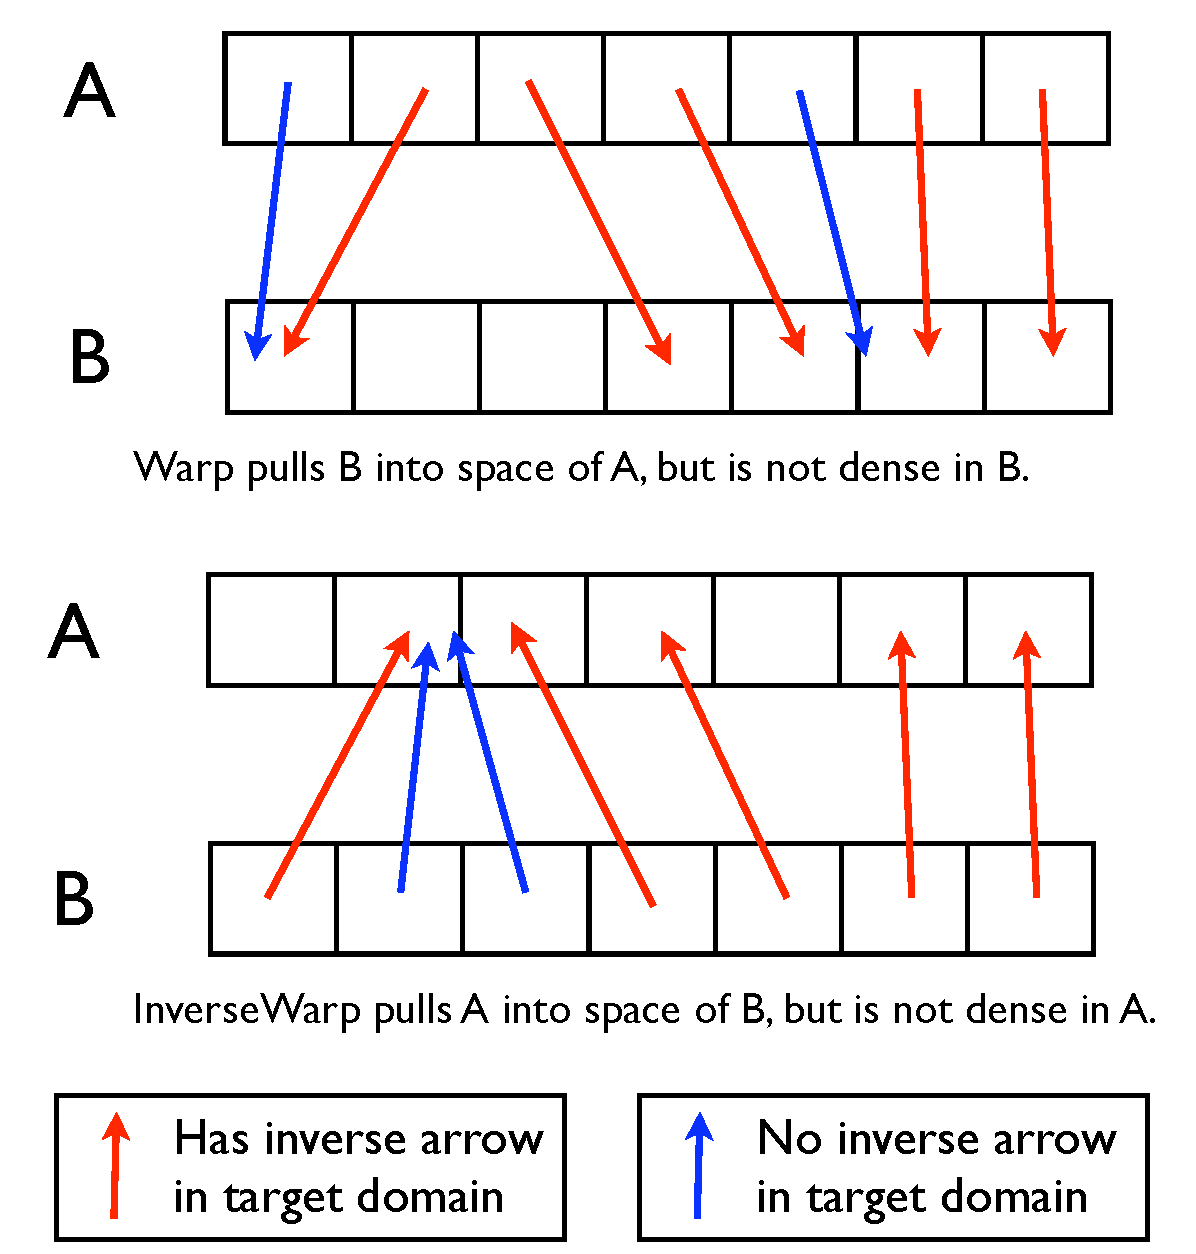
\includegraphics[width=0.75\textwidth]{Figures/DeformationsInDigitalDomain.pdf} 
\itkcaption[Digital Invertibility]{Digital invertibility presents some limitations. 
Here, we see that invertibility is not exact but is gained only by interpolation.  
Thus, in three-dimensional scenarios in particular, there are fundamental limits to the 
degree of invertibility that may be achieved.  The second and third voxels -- from left -- 
in image A undergo an expansion by a factor of 2.  That is, under the mapping, 
2 voxels are mapped to 4.  This gives the definition of the Jacobian -- computed 
by  ANTsJacobian -- which is a unitless measure defined by the 
ratio of volumes.  Thus, $\mathcal{J}(\x)=V(\phi(\x))/V(\x)$ where $V$ represents 
the volume operation and $\x$, here, may be a small object.  Thus, if $\phi$ -- the mapping -- 
causes expansion, then $\mathcal{J}(\x) > 1$. }
\vspace{-0.1in}
\label{fig:inv}
\end{figure}  
A few important notes follow. 
(1) Deformation directionality: Warps/deformations applied to images occur in the opposite direction from warps/deformations applied to points. That is, if we map image B to A using 
\lstinputlisting[style=mystyle,linerange={3-1000}]{examplesandtests/Ex4.sh}
 then we get a deformation called \texttt{OUTPUT1Warp.nii.gz} and an affine transform called \texttt{OUTPUT0GenericAffine.mat} . 
This composite mapping -- when applied to B -- will transform B into the space of A. 
However, if we have points defined in B that we want to map to A, 
we have to use \texttt{OUTPUT1InverseWarp.nii.gz} and the inverse of \texttt{OUTPUT0GenericAffine.mat}.  
This is because the domain and range of the map's definition need to be dense in a way that is appropriate for the data type. 
Figure~\ref{fig:inv} illustrates the concept. 
(2) Older Image Formats: older image formats (e.g. Analyze) may not
have proper origin/offset/direction support! In these cases, we
recommend converting to nii and verifying that data overlays properly.
(3) Transorm Composition: Composition of transforms may be achieved with
\texttt{antsApplyTransforms}.  (4) Warping with inverses and concatenations --
viable when using diffeomorphisms -- are described in
figure~\ref{fig:warp}.
 \begin{figure}
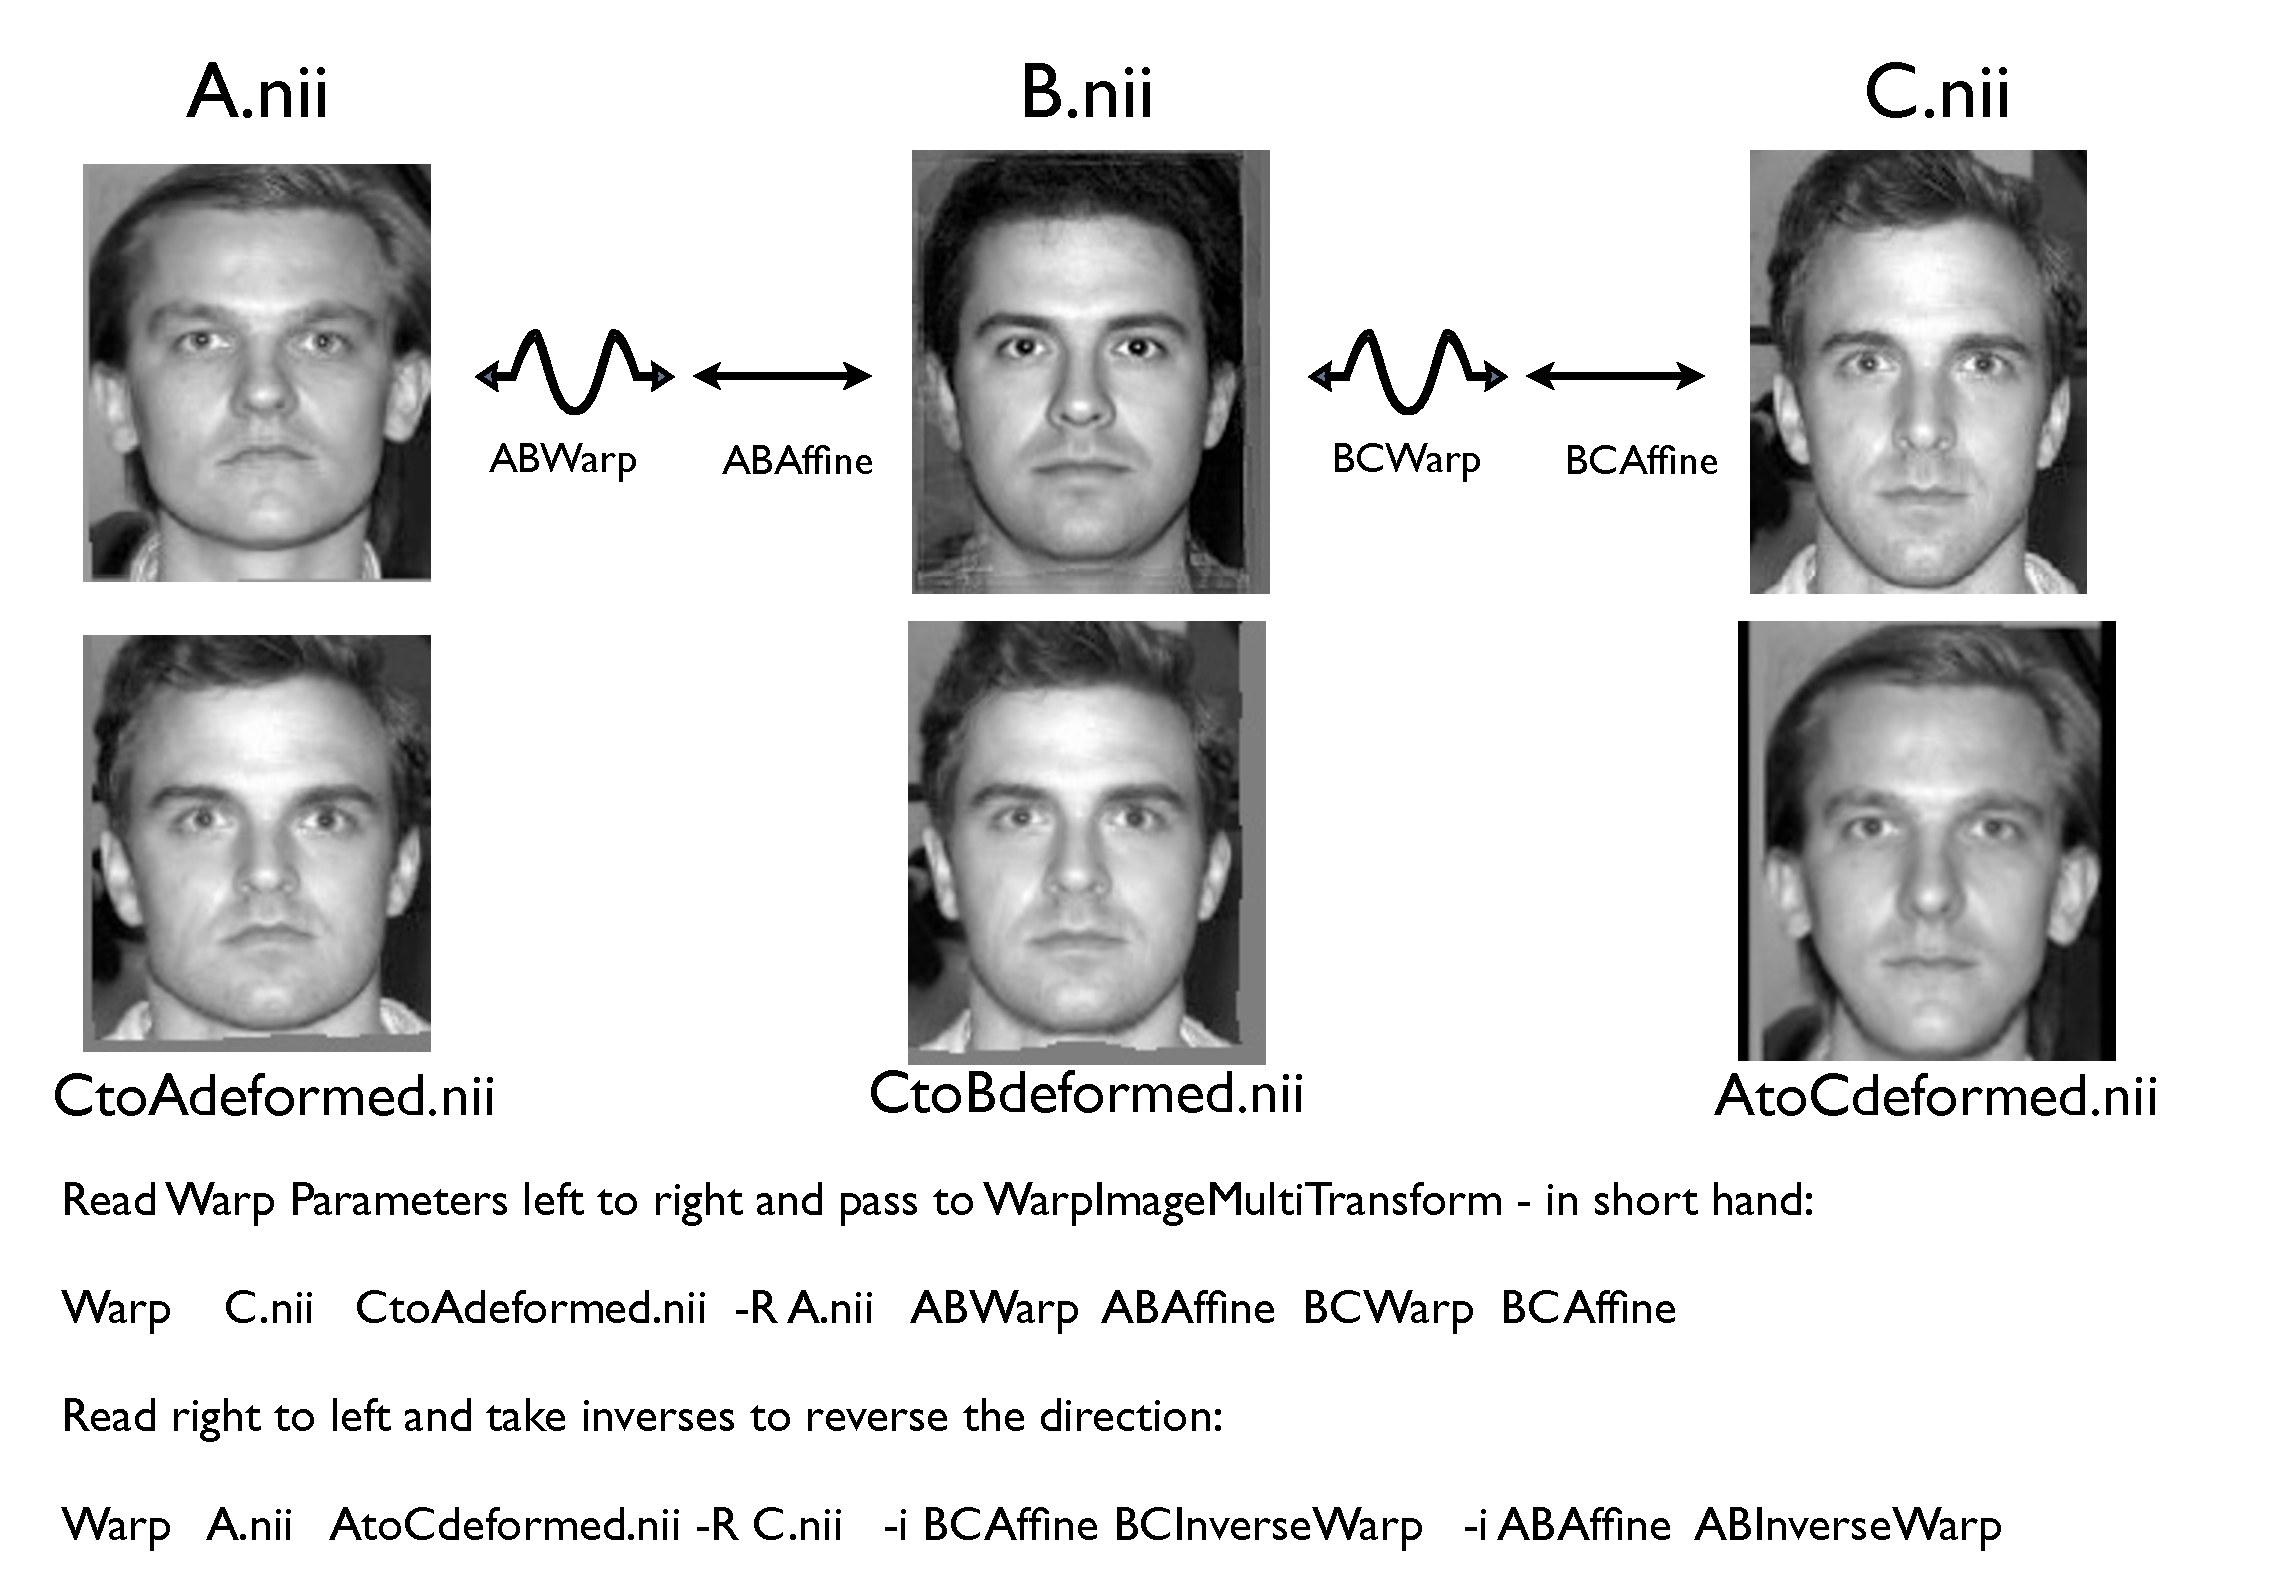
\includegraphics[width=0.9\textwidth]{Figures/ANTSSyntax2.pdf} 
\itkcaption[ANTs Warping]{Here, we detail how one applies 
a deformation and associated inverses.  We also see how 
antsApplyTransforms can be used to concatenate a series 
of transformations.   In brief, read parameters left to right, then
pass to \texttt{antsApplyTransforms}.  To warp $C$ to $A$ (in
short-hand): \texttt{antsApplyTransforms -t  ABWarp -t ABAffine -t
BCWarp -t BCAffine}.   Use the inverse composite transform to warp $A$ to $C$ (in
short-hand): 
\texttt{antsApplyTransforms -t  $[$BCAffine,1$]$ -t BCInverseWarp -t
  [ABAffine,1] -t ABInverseWarp} 
.  Note, to focus on the key idea, we dropped the other parameters needed for a proper
\texttt{antsApplyTransforms} call.}
\vspace{-0.1in}
\label{fig:warp}
\end{figure}

\noindent{\bf Diffeomorphic Transformations.}  The elastic 
mapping space -- as indicated above -- may prove inadequate 
for some large deformation mapping scenarios.  Figures~\ref{fig:antshier} 
illustrate the changing performance one may get in switching from affine 
to elastic to diffeomorphic normalization.  
\begin{figure}
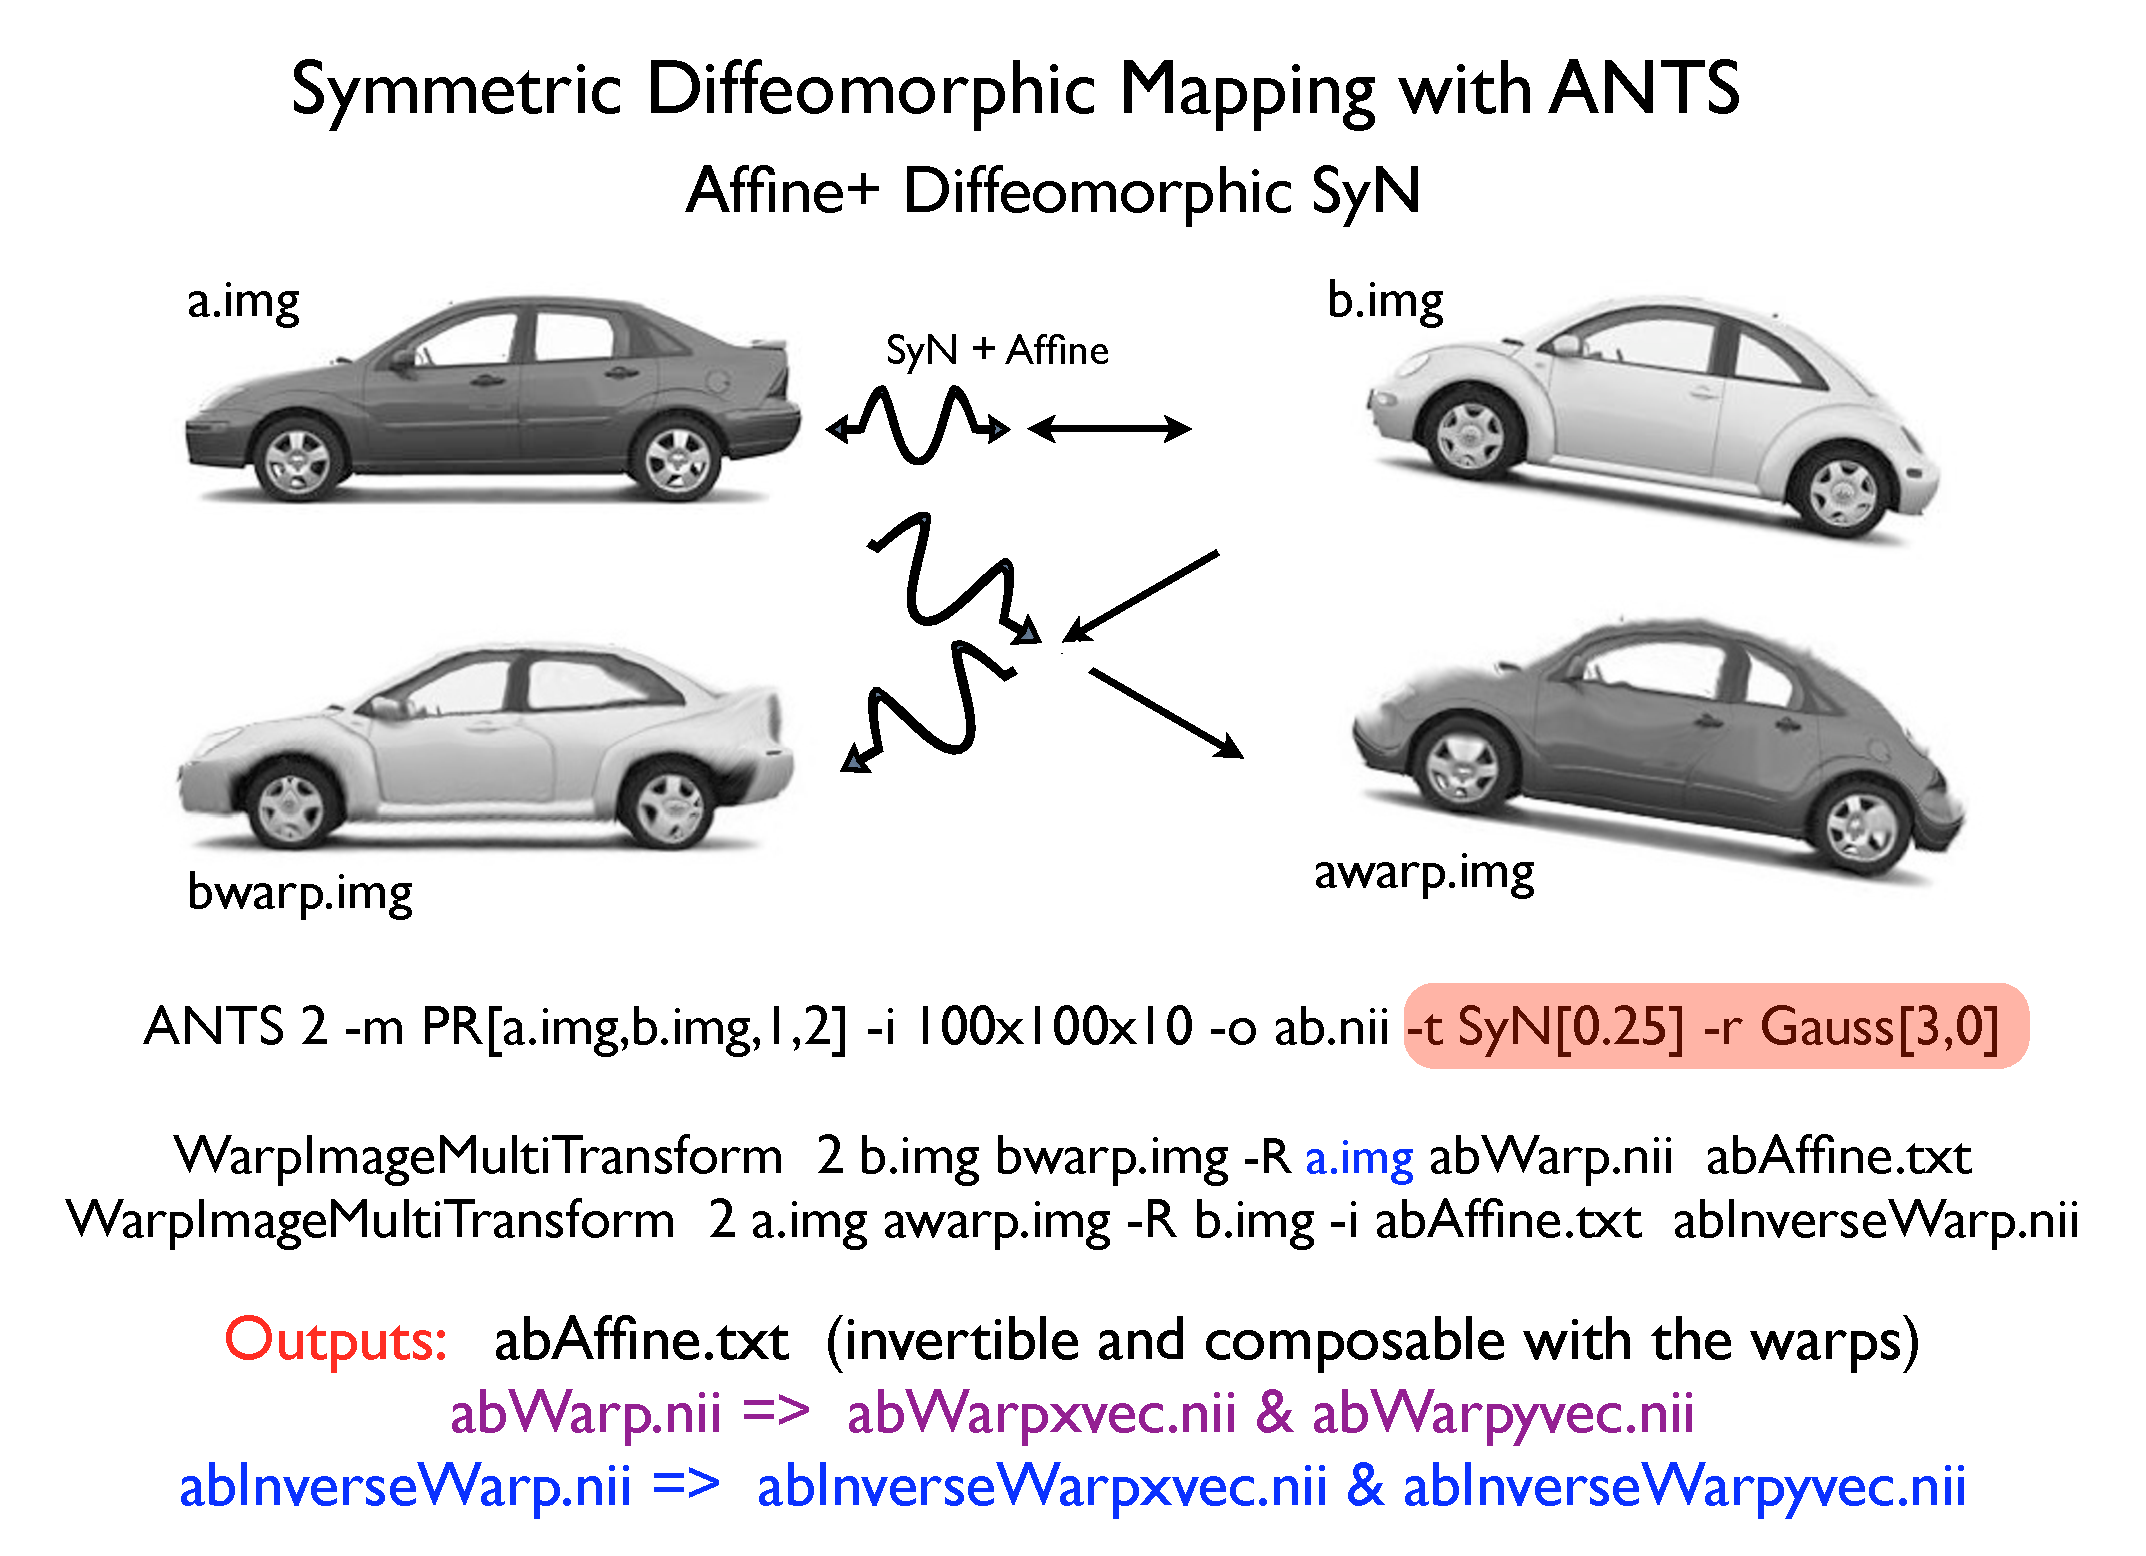
\includegraphics[width=0.9\textwidth]{./Figures/ANTSsyn.pdf} 
\itkcaption[ANTs Symmetric Normalization]{This example shows the
  benefit of the symmetric normalization model -- invertibility,
  symmetry, highly deformable and accurate registration.  This example
may be recreated by the reader via:  \href{http://stnava.github.io/cars/}{http://stnava.github.io/cars/}.}
\vspace{-0.1in}
\label{fig:antssyn}
\end{figure}
Figure~\ref{fig:antssyn} shows 
how one may use ANTs to achieve a state-of-the-art diffeomorphic mapping. 
The ANTs diffeomorphic model chosen for this example -- symmetric normalization \cite{Avants2008b,Kim2008} -- 
is invariant to the order of the input images (although the affine mapping is not).  
An additional advantage of the diffeomorphic model over the elastic model is 
that both forward and inverse transformations are computed thus allowing one 
to deform fixed to moving and also moving to fixed.   The transformation model 
chosen here -- \texttt{SyN[0.1,3,0.0]} -- may be replaced with other 
diffeomorphic transformation models.  The most general is global-in-time SyN via \texttt{SyN[0.1,3,0.0]}   , 
where the time step for integration is 0.01 (lower is more accurate).  A fast approximate 
solution may be gained through 
exponential mapping via \texttt{Exponential[0.1,3,0.5,10]} , where 10 integrations points are used. 
Update schemes for diffeomorphic optimization are similar to the elastic case 
and are described elsewhere \cite{Avants2008b}.   

\subsection{ANTs similarity terms}
Here is a script that will let you experiment with different similarity term 
and transformation model combinations.  A few are listed, with parameters 
that are a reasonable starting point.  This example implements an
elastic mapping driven by neighborhood cross-correlation and initialized by mutual information affine:
\lstinputlisting[style=mystyle,linerange={3-1000}]{examplesandtests/Ex4.sh}
This example implements a greedy syn mapping that includes elastic regularization and is driven by mutual
information and initialized by global correlation with a similarity transform:
\lstinputlisting[style=mystyle,linerange={3-1000}]{examplesandtests/Ex5.sh}

\noindent\textbf{Using multiple metrics to drive registration.}
This example uses smoothing without downsampling (ie scale-space) and
implements a greedy syn driven by two unequally weighted similarity metrics and no affine mapping:
\lstinputlisting[style=mystyle,linerange={3-1000}]{examplesandtests/Ex6.sh}
Convergence occurs under two conditions: (1) either the maximum number of 
iterations are reached at a given optimization level or (2) the slope 
of the change in the optimization objective is negative or very small. 


\subsection{Choosing a metric}
ANTS supports both volumetric registration and point set registration. The image / point set similarity metrics in ANTS are unified in the form of a function on the images or the point sets:       $$\textbf{Simlarity}[\textbf{fixedImage}, \textbf{movingImage}, \textbf{weight}, \textbf{parameters}].$$
        
The similarity type for the deformation transformation is specified by \verb -m  option, which contains two parts: simarity type and the parameters inside the brackets. (Note: no white spaces exist between parameters.) The possible similarity metrics for volumetric images are: 
\begin{itemize}
    \item Cross correlation estimate:  \verb"-m CC[fixedImage,movingImage,weight,radius]". This metric works well for intra-modality image registration. For exxample, \verb"-m CC[fixed.nii,moving.nii,1,5]" specifies:
    \begin{itemize}
        \item the fixed image: fixed.nii
        \item the moving image: moving.nii             
        \item weight for this metric is 1 (i.e. only this metric drives the registration).      
        \item the region radius for computing cross correlation is 5
    \end{itemize}

    \item Mutual information: \verb"-m MI[fixedImage,movingImage,weight,number-of-histogram-bins]". This metric works both well for intra-modality and inter-modality image registration. For example, the first three parameters in \verb"-m MI[fixed.nii,moving.nii,1,32]" is similar to the example above in cross correlation, except that the last parameter means that the number of bins in computing mutual information is 32.

    \item PR: \verb"-m PR[fixedImage,movingImage,weight,radius]". This metric works for intra-modality image registration and some inter-modality cases. This metric is a strict implementation of correlation whereas CC estimates correlation-like optical flow. The meaning of parameters are similar to cross correlation.

    \item Mean square difference: \verb"-m MSQ[fixedImage,movingImage,weight,0]". This metric works for intra-modality image registration. The last parameter \verb"0" is a padding value of no real meaning. For example, \verb"-m MSQ[fixed.nii,moving.nii,1,0]". 

\end{itemize}

ANTS also support registration of point sets. The supported formats for point sets can be found in I/O section. The similarity metrics for point sets are:
\begin{itemize}
    \item Point set expectation: 
     \begin{verbatim}
-m PSE [fixedImage,movingImage,fixedPoints,movingPoints,weight,
pointSetPercentage,pointSetSigma,boundaryPointsOnly,
kNeighborhood,PartialMatchingIterations=100000]
    \end{verbatim}
    \begin{itemize}
        \item \verb"fixedImage": defines the space domain of the fixed point set.
        \item \verb"movingImage": defines the space domain of the moving point set.
        \item \verb"fixedPoints/Image": defines the coordinates of the fixed point set or label image. It can be an image with discrete positive labels, a VTK format point set file, or a text file. Details can be found in I/O section (TODO).
        \item \verb"movingPoints/Image": defines the coordinates of the moving point set or label image. 
        \item \verb"weight": weight for this metric. \verb"1" means that only this metric drives the registration.
        \item \verb"pointSetPercentage": the percentage of points to be randomly sampled used in the registration.
        \item \verb"pointSetSigma": the standard deviation of the Parzen window used to estimate the expectation. 
        \item \verb"boundaryPointsOnly":  \verb"1" (or ``true'') means only the boundary points in the label image is used to drive registration.
        \item \verb"kNeighborhood" is a positive discrete number. The first $k$ neighbors are used to compute the deformation during the registration. 
        \item \verb"PartialMatchingIterations" controls the symmtry in the matching. This option assumes the complete labeling is in the first set of label parameters ... more iterations leads to more symmetry in the matching  - 0 iterations means full asymmetry 
    \end{itemize}

    \item Jensen-Tsallis BSpline
    \begin{verbatim}
-m JTB[fixedImage,movingImage,fixedPoints,movingPoints,weight,
pointSetPercentage,pointSetSigma,boundaryPointsOnly,kNeighborhood,alpha,
meshResolution,splineOrder,numberOfLevels,useAnisotropicCovariances] 
    \end{verbatim}
    \begin{itemize}
        \item \verb"fixedImage": defines the space domain of the fixed point set.
        \item \verb"movingImage": defines the space domain of the moving point set.
        \item \verb"fixedPoints": defines the coordinates of the fixed point set. It can be an image with discrete positive labels, a VTK format point set file, or a text file. Details can be found in I/O section (TODO).
        \item \verb"movingPoints": defines the coordinates of the moving point set.
        \item \verb"weight": weight for this metric. \verb"1" means that only this metric drives the registration.
        \item \verb"pointSetPercentage": the percentage of points to be randomly sampled used in the registration.
        \item \verb"pointSetSigma": the sigma for the Parzen window used to estimate probabilities.  
        \item \verb"boundaryPointsOnly": [TODO] \verb"1" (or ``true'') means only the boundary points in the point sets are used to drive registration.
        \item \verb"kNeighborhood" is a positive discrete number. The first $k$ neighbors are used to compute the deformation during the registration. 
        \item \verb"alpha"
        \item \verb"meshResolution"
        \item \verb"splineOrder"
        \item \verb"numberOfLevels"
        \item \verb"useAnisotropicCovariances"
    \end{itemize}

\end{itemize}

In current implementation, the affine registration only supports two types of similarity metrics on volumetric images, which are specified using \verb"--affine-metric-type":
\begin{itemize}
    \item Mutual information, specified as \verb"--affine-metric-type MI". This usually works for both inter and intra-modalities in 3D. Also, the options used in computing mututal information in affine registration can be specified as \verb"--MI-option N1xN2". The first parameter \verb"N1" specifies the number of bins. The second parameter \verb"N2" specifies the number of samples. For example: \verb"--MI-option 32x8000".

    \item Mean square difference, specified using \verb"--affine-metric-type MSE". There is no options for this metric.
\end{itemize}

Fig. \ref{fig:metric_example} shows the registration result using intensity difference with the following command:
\begin{verbatim}
ANTS 2 -m MSQ[r16slice.nii,r64slice.nii,1,0] -r Gauss[3,0] -t SyN[0.5] -i 50x50x30
\end{verbatim}

%        \begin{wrapfigure}{r}{0.5\textwidth}
\begin{figure}
    \label{fig:metric_example}
    \centering
    \begin{tabular}[h]{c|c|c}
%        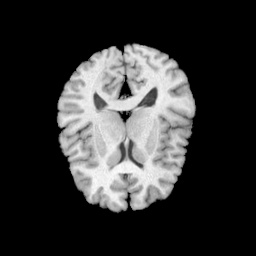
\includegraphics[width=0.16\textwidth]{Figures/r16slice.jpg} &
%        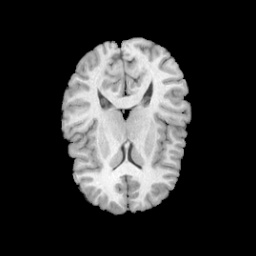
\includegraphics[width=0.16\textwidth]{Figures/r64slice.jpg} &
 %       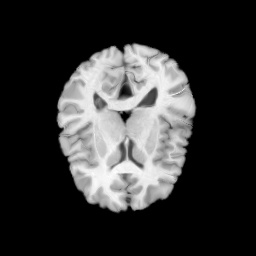
\includegraphics[width=0.16\textwidth]{Figures/resMSQ.jpg} \\
        fixed image &
        moving image & 
        MSE  \\
    \end{tabular} 
    \itkcaption{registration using mean square intensity difference}
\end{figure}
    %    \end{wrapfigure}
Here is also an example script to register a pair of images using mean square intensity difference and computing the metrics of the registration image.
\begin{verbatim}
#use intensity difference with radius 0 -- radius no effect on intensity difference
ANTS 2 -m MSQ[r16slice.nii,r64slice.nii,1,0] -r Gauss[3,0] -t SyN[0.5] -i 50x50x30
WarpImageMultiTransform 2 r64slice.nii resMSQ.nii Warp.nii Affine.txt
MeasureImageSimilarity 2 0 r16slice.nii resMSQ.nii metricexamplelog.txt
MeasureImageSimilarity 2 1 r16slice.nii resMSQ.nii metricexamplelog.txt
MeasureImageSimilarity 2 2 r16slice.nii resMSQ.nii metricexamplelog.txt
ConvertToJpg resMSQ.nii resMSQ.jpg
\end{verbatim}

\lstinputlisting[style=mystyle,linerange={3-1000}]{examplesandtests/Ex7.sh}


\subsection{Notes on basic brain mapping}
There is ``maximally robust'' brain mapping and there is ``fast''
brain mapping.  These two goals may, at times, be adversarial.  
A simple and ``fast'' brain registration example is here
\href{http://stnava.github.io/BasicBrainMapping/}{http://stnava.github.io/BasicBrainMapping/}.
This example shows a non-optimized use of \texttt{antsRegistration}
and compares it to the case where the registration is \textit{masked}
in order to focus the registration.  Such strategies may be used for
brains with missing data e.g. lesions.

\subsection{Normalization across different modalities: E.g. DTI}
The \texttt{ImageMath} program -- via TensorFA and TensorMeanDiffusion -- 
may derive scalar images from DTI.  Such images may be used to 
distortion correct DTI to T1 or to map DTI together.   See the 
ANTS/Scripts program called \texttt{antsIntermodalityIntrasubject.sh}
for an example of how one might implement the strategy outlined in \cite{Tustison2014}.   Figure~\ref{fig:dterr} shows what might 
happen if your tensor entries are stored in the wrong order. 
ANTs expects the nifti standard ordering of the DT six vector.
\begin{wrapfigure}{r}{0.5\textwidth}
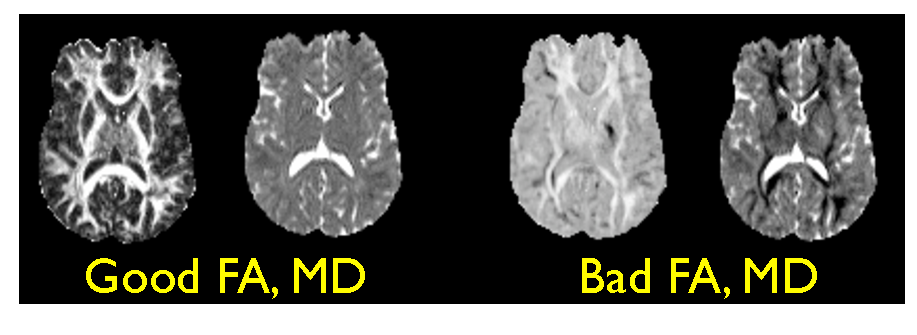
\includegraphics[width=0.5\textwidth]{Figures/dtiordererr.pdf} 
\itkcaption[DT Entry Error]{The FA and mean diffusion of the tensor may be corrupted, 
as at right, if the order of the DT entries is wrong.}
\vspace{-0.1in}
\label{fig:dterr}
\end{wrapfigure}  
\subsection{Multivariate normalization with ANTs}
\begin{figure}
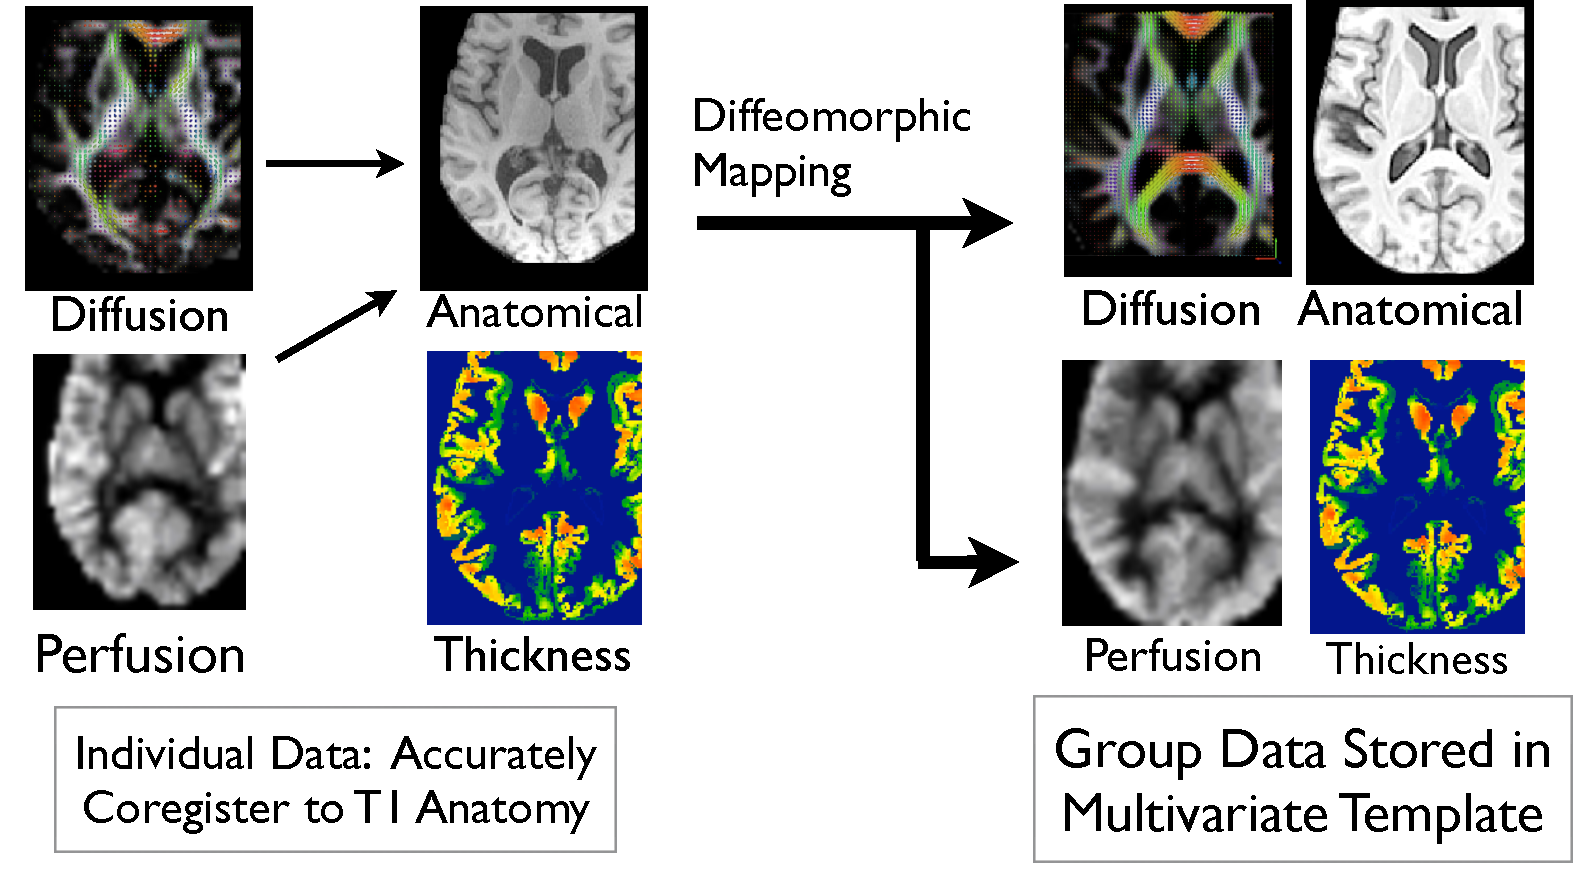
\includegraphics[width=0.9\textwidth]{Figures/multivariatenorm.pdf} 
\itkcaption[Multivariate Normalization]{The current version of ANTs 
may perform normalization of multiple modalities by combining {\em intrasubject, intermodality} mappings with {\em intersubject, intramodality} maps to a 
group template.  In brain imaging, the intersubject maps are usually guided by the T1 component.}\vspace{-0.1in}
\label{fig:mvnorm}
\end{figure}
Multivariate normalization may be performed in two ways with ANTs.  
First, as shown in figure~\ref{fig:mvnorm}, intra-subject mappings may 
be used to conform all modalities into a common subject space defined by 
the ``anchor'' modality.  In brain imaging, this is usually the T1 component.  

A second type of multivariate normalization is able to use the T1 and DTI components 
directly in the optimization of the mapping.  We usually assume that one has resampled data to the space of T1.
In this case, dense features within white matter are gained by using the DT component  
in addition to the T1 component.   One might also weight the T1 CC metric slightly more 
than the FA CC metric, 1.25 vs. 1.0.  {\em The convergence criterion for 
the multivariate scenario is a slave to the {\bf last} metric you 
pass on the ANTs command line}.

\subsection{Notes on large deformation mapping} 
Figure~\ref{fig:large} defines what one might expect from a 
high-resolution, large deformation, successful normalization.  
Major and many minor features are well aligned between 
these images to an extent that is approaching the limits 
allowable by biological variation.  
\begin{figure}
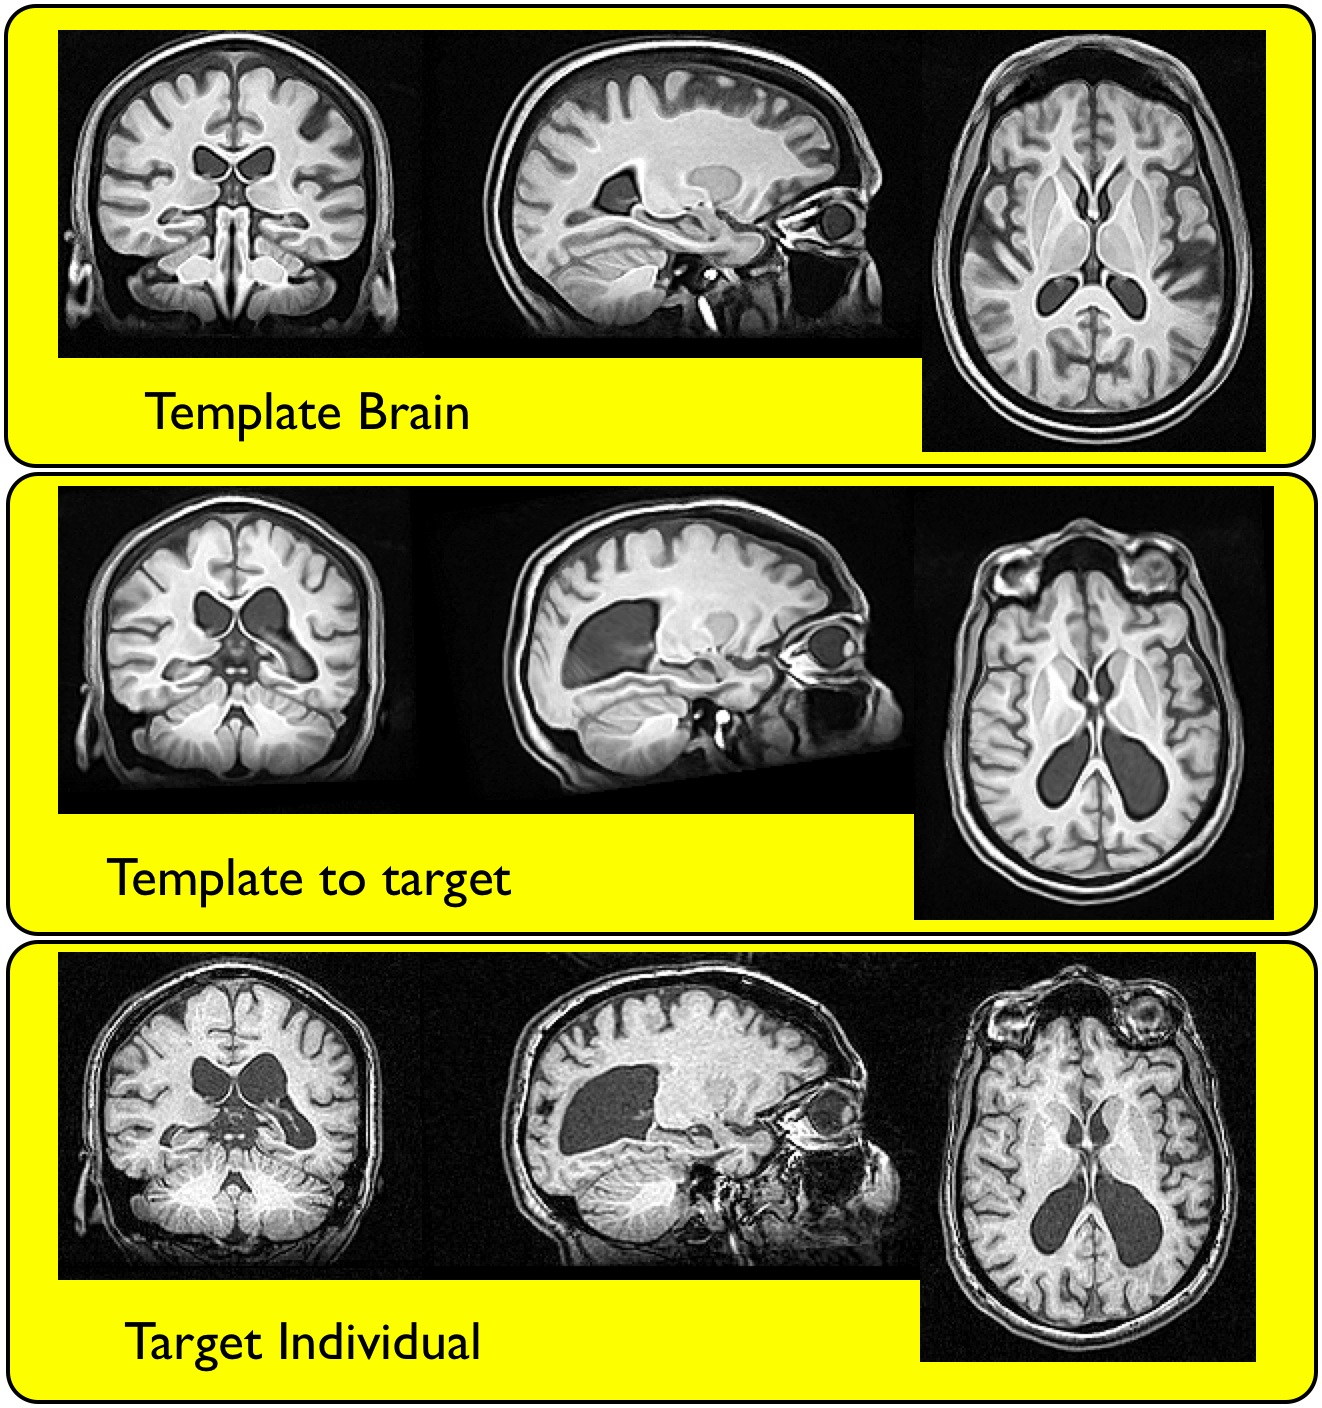
\includegraphics[width=0.9\textwidth]{Figures/ANTSLargeDef.jpg} 
\itkcaption[ANTs LargeDeformation]{ANTs succeeds in a challenging 
normalization scenario.  Comparing the template mapping to the
individual shows that much of the cortex is well-aligned, as is the
hippocampus, despite the relatively large difference between the
initial template and the target.  Here, one might note a limitation of
whole brain mapping: occipital lobe sulcal variation is highly
idiosyncratic and extremely difficult to capture, in particular when
there is such severe atrophy nearby.
}
\label{fig:large}
\end{figure}

\noindent{\bf Turning ``Failures" into Successes:} 
Below are some pointers to follow if you are unable to recreate such normalization quality.  
Usually, reasons for registration failure are one of a very few things: 
\begin{enumerate}
\item The initialization is so off mark that affine registration fails -- thus meaning all subsequent deformable registration will not be meaningful.
\item The information within headers is inconsistent e.g. origins are defined in different ways, the ``directions" are not correct or some combination of these.    The PrintHeader executable can help one in debugging this type of problem.  
\item  The similarity or transformation model is inappropriate or has too small a capture region for the problem. 
\end{enumerate}

Large deformation mapping is challenging not only because of the
amount of deformation, but also because the ``true'' solution becomes
more difficult to find as the distance between images increases.
Keeping this in mind, fixing registration failures means 1. better
initialization or 2. increasing the capture range of the registration. 
Key changes may include more multi-resolution levels, increasing the radius of the neighborhood
correlation, more dense or more focused sampling and/or 
allowing more iterations during the optimization.  
Note: the coarsest levels of the computation take only about
10 percent of the time (a few minutes depending on the machine)
but account for the large majority of the shape variation.  Therefore,
inspecting results after only low resolution registration is performed
can save significant time and make parameter optimization more rapid.

\subsection{Optimal template construction with ANTs}
A useful script for setting up optimal template construction
 is available in ANTs/Scripts.  This method is described in \cite{Avants2004,Avants2006d,Kim2008,Yushkevich2009,Avants2009c}, 
where more recent publications are more descriptive and incorporate 
more recent features and optimization strategies. 
Two versions of this algorithm are available : serial and parallel.  
Data and a script for building an average face template is available 
at \href{http://ntustison.github.io/TemplateBuildingExample/}{http://ntustison.github.io/TemplateBuildingExample/}.  Two key points about optimal templates:
1. The outcome stabilizes at around ten images, for most populations.
That is, if we randomly select images from individuals within the same 
demographic distribution, we will end up with very similar average images.  
2.  Optimality, for the ANTs-SyN approach, is defined by the minimum shape 
and appearance distance image. 
See the template page for some examples of this and users may 
contact ANTs developers for previously derived template 
images that may be useful. 

The goal of template construction is to derive a ``most representative'' single image from a population. 
The steps are: 
\begin{figure}
\center 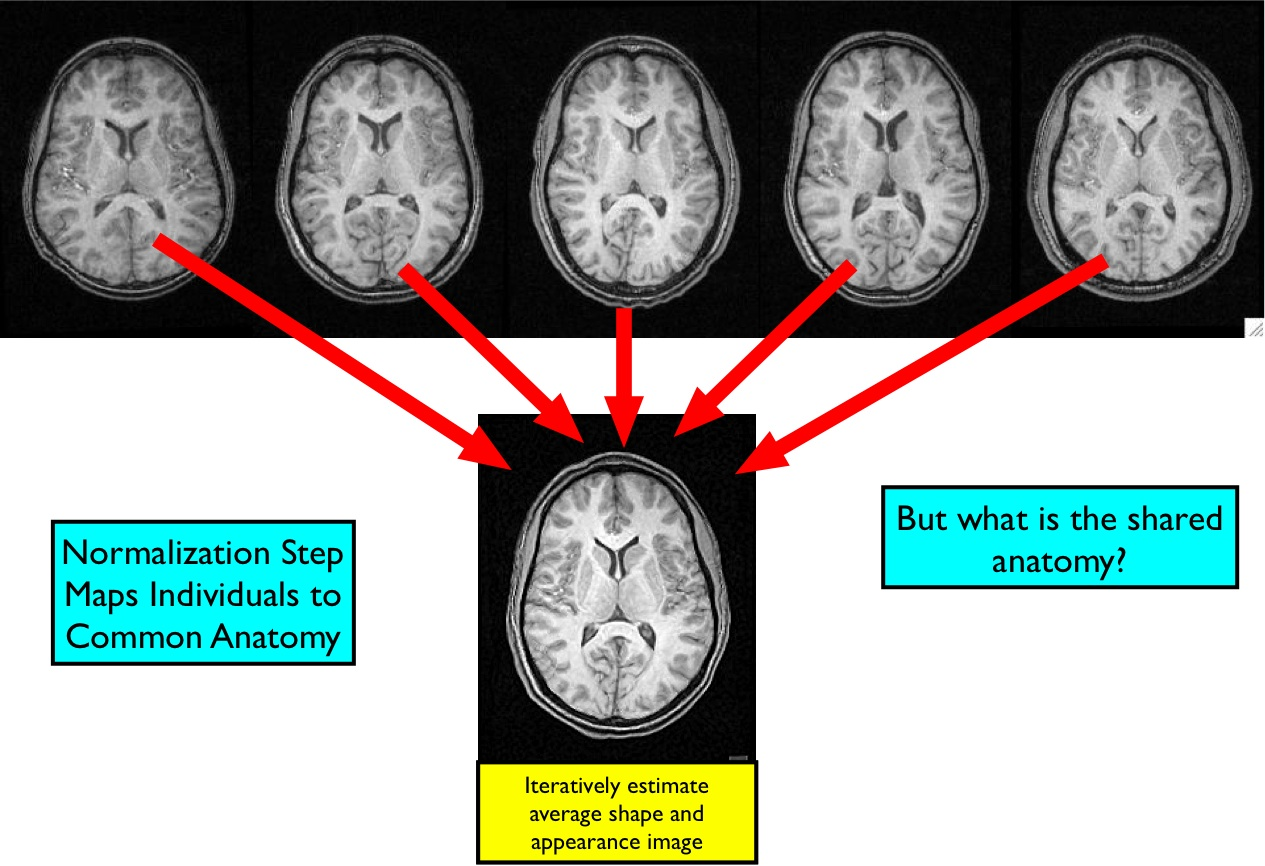
\includegraphics[width=0.7\textwidth]{Figures/templateex.jpg} 
\itkcaption[ANTs Optimal Template]{This example may be recreated by
  the user via \href{http://ntustison.github.io/TemplateBuildingExample/}{http://ntustison.github.io/TemplateBuildingExample/}. 
The shared anatomy -- 
across this dataset -- is recovered in the derived optimal template.}
\label{fig:template}
\end{figure}
\begin{enumerate}
\item   Make a directory for your data.   Copy or link all the images into it.
\item  On the command line, within that directory, run the following command: 
\texttt{bash}  \texttt{antsMultivariateTemplateConstruction2.sh}  to get usage. 
\item   Follow the example outlined in the TemplateBuildingExample
  above but modified for your own data and needs. 
\item The script should exit and store a log of what happened. 
\item If there is a problem, check the path to the programs, the fact that all the images you want to use are being 
listed and that the template output name is ok.  
\end{enumerate}
The script is fairly easy to alter so that you can send the whole thing to distributed computing. 
Typically, one would use voxbo or the qsub program available in the Sun Grid Engine.  This 
is what is done in \texttt{antsMultivariateTemplateConstruction2.sh}.  
Figure~\ref{fig:template} shows the data and a result similar to what may be recreated by the user.

\subsection{2D to 3D registration}
There has been much discussion of this on the ITK and ANTs lists.
What it boils down to is this:  the 2D to 3D (or vice versa) problem
is inherently asymmetric and (very) ill-posed.  So, we currently
recommend, as a start, running \texttt{antsRegistrationSyNQuick.sh} in both
directions and seeing which works better.   Both directions means pass
the 2D image to the \texttt{-f} option and compare to the result of passing
the 2D image to the \texttt{-m} option, noting that the resulting transforms are NOT inverses of
each other.

\subsection{More ANTs examples}
The paper
\href{http://journal.frontiersin.org/Journal/10.3389/fninf.2014.00044/abstract}{http://journal.frontiersin.org/Journal/10.3389/fninf.2014.00044/abstract}
shows or links to several more examples.  Some of these include
morphometry.  
Many other examples are available in the literature \href{http://scholar.google.com/citations?user=ox-mhOkAAAAJ&hl=en}{Google
  Scholar Search}.


\newpage
\section{Image segmentation and labeling}
ANTs has tools for both tissue based segmentation and prior-based segmentation that 
leverages spatial priors, usually based on a template mapping.  
\subsection{Basic segmentation}
A suite of segmentation algorithm approaches are available by
combining the \texttt{Atropos} tool with various feature images,
priors and objective functions.  But let's show a simple example
first. We apply k-means segmentation to 2D data (the call is the same
in 3D except for the dimensionality flag). 
\lstinputlisting[style=mystyle,linerange={3-1000}]{examplesandtests/Ex8.sh}
The parameter \texttt{4} indicates 4 tissues plus background are
sought.  The \texttt{mask} identifies the region that will be segmented. 
There are no prior images available to guide the segmentation.
Representative output is shown 
in figure~\ref{fig:seg} and -- with priors -- in figure~\ref{fig:seg2}.
\begin{figure}
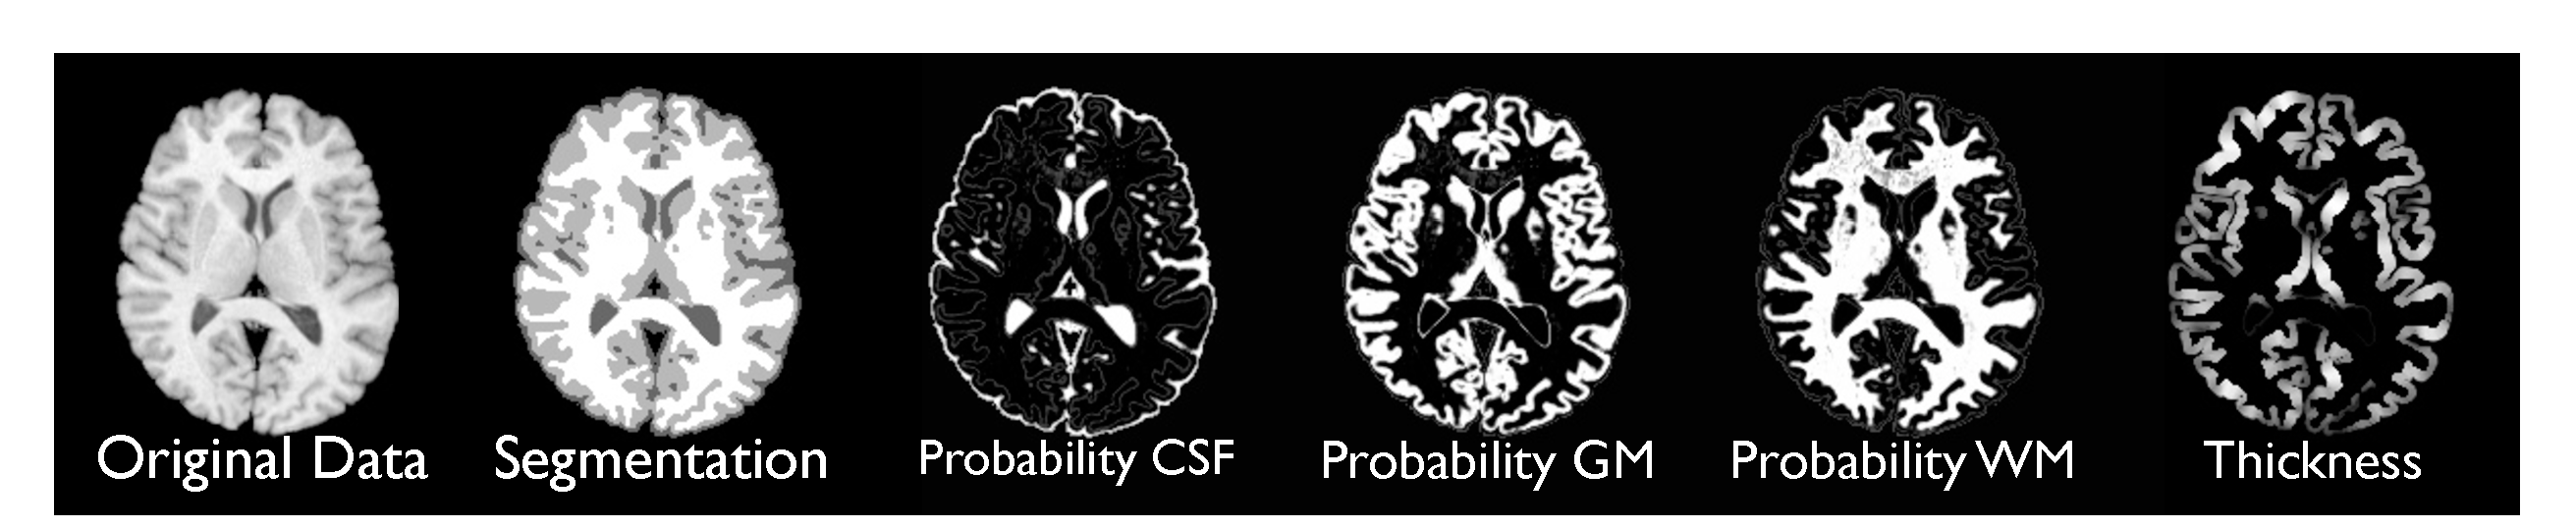
\includegraphics[width=1\textwidth]{Figures/segmentation.pdf} 
\itkcaption[ANTs Segmentation]{ANTs provides basic 
Markov Random Field regularized Gaussian model tissue segmentation. 
The ANTs program N4 or N3BiasFieldCorrection is very valuable as preprocessing 
for this naive approach to segmentation.   The last panel -- far right -- 
shows the thickness derived from the white matter and gray matter 
probabilities where a prior on thickness was used to prevent thickness
overestimation.   Thickness was derived with DiReCT \cite{Das2009}
which is called \texttt{KellyKapowski} in its implementation.  
}
\label{fig:seg}
\end{figure}
\subsection{Prior and template-based image segmentation}
The same algorithm may be augmented 
to perform Prior-based segmentation.  
The parameter \texttt{4 indicates 3 tissues plus background are sought}.  The \texttt{0.5} indicates 
we weight the priors equally as the data term and use a spatially varying set of Gaussians 
to estimate the segmentation.  In this way, data from the priors may be used to modify 
and guide the segmentation in a locally varying way, accomodating for both inhomogeneity 
and the different imaging signature that different tissues provide.   Prior images should be 
of the same size and dimension as the input data and should have intensities in the range $[0,1]$.
\lstinputlisting[style=mystyle,linerange={3-1000}]{examplesandtests/Ex9.sh}
\begin{figure}
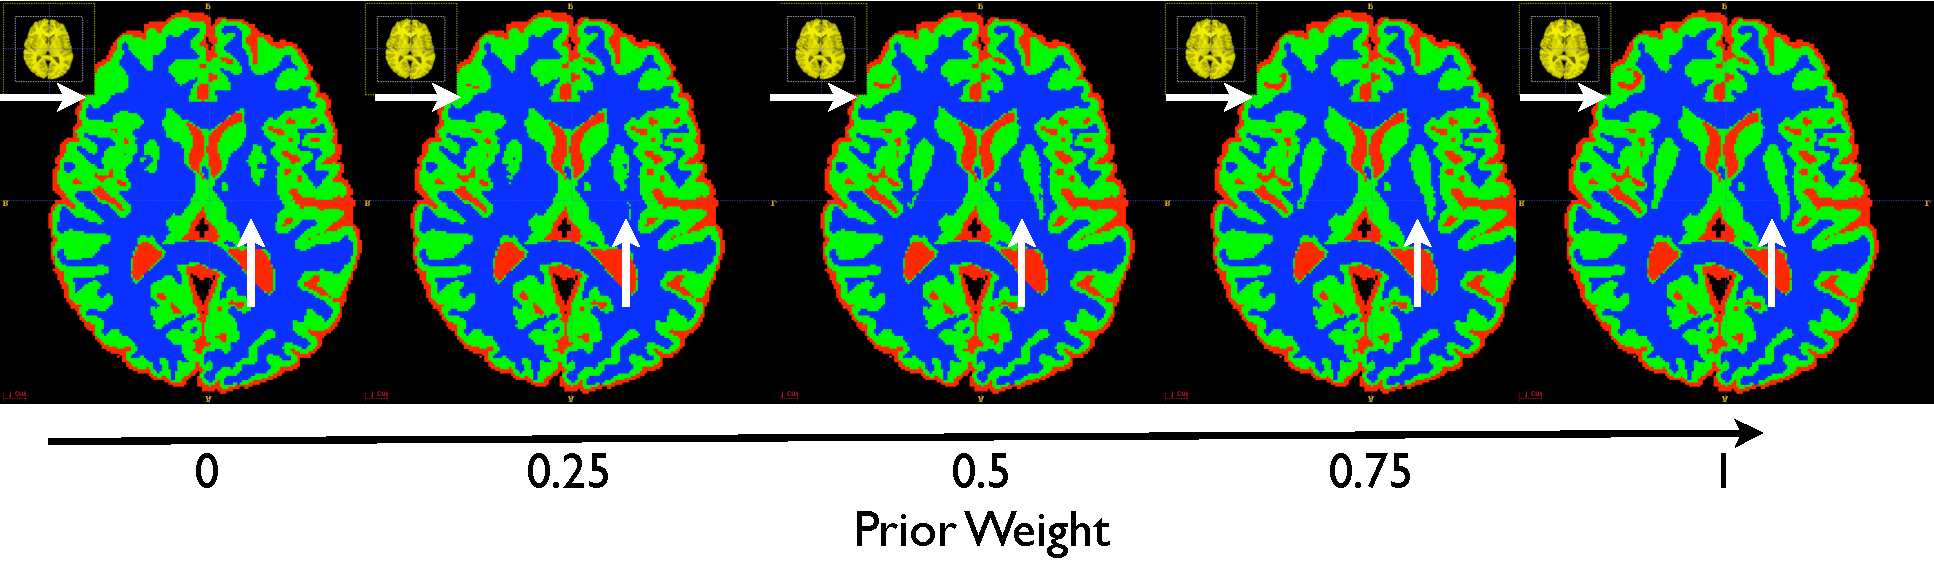
\includegraphics[width=1\textwidth]{Figures/segmentation2.pdf}
\itkcaption[ANTs Segmentation]{ANTs extends basic Markov Random Field
  regularized Gaussian model tissue segmentation to include priors,
  which allow spatially varying tissue models to determine
  segmentation.  The ANTs program N3BiasFieldCorrection is less
  critical as preprocessing when using this approach to segmentation.
  Here, we see the improvement in segmentation as the locally varying 
  prior models are weighted more heavily.  
  The last panel -- far right -- shows the segmentation derived from
  data driven with an initialization founded purely on prior models 
  based on template mapping.  The prior model brings out the caudate 
and some CSF -- highlighted by arrows -- as their weight increases. 
}
\label{fig:seg2}
\end{figure}
This listing also shows how Atropos becomes instantaneously
multivariate with more input feature images and that the likelihood
model \texttt{ -k } is also flexible.
More detailed examples are here:
\href{https://github.com/ntustison/antsAtroposN4Example}{https://github.com/ntustison/antsAtroposN4Example}
with brain extraction here: \href{https://github.com/ntustison/antsBrainExtractionExample}{https://github.com/ntustison/antsBrainExtractionExample}.

\subsection{Cortical thickness}
Two forms of cortical thickness estimation from probability maps are available 
in ANTs: first, the traditional Laplacian cortical thickness estimation and, second, 
the more recently developed Diffeomorphic Registration-based Cortical Thickness 
(DiReCT) \cite{Das2009}.  Both methods estimate thickness of an object 
from probability or binary images that define object boundaries.  This tool 
is mainly of interest in brain mapping and cardiac imaging for morphometric 
studies.  Cortical thickness, for instance, is known to correlate with language 
development and IQ in adolescents.  The laplacian approach to 
cortical thickness may be used via the program LaplacianThickness, 
which implements the method described in ``Three-dimensional mapping of cortical thickness using Laplace's Equation'' by 
Jones, et al \cite{}.  Super-sampling 
and controlling segmentation accuracy for input to this program is up 
to the user.  Otherwise, the Laplacian method may grossly overestimate 
thickness in closed sulci.  See the full example:  \href{https://github.com/ntustison/antsCorticalThicknessExample}{https://github.com/ntustison/antsCorticalThicknessExample}.

\begin{comment}
\subsection{User/label-guided normalization for hippocampus mapping}
See the link for details on hippocampus labeling:
\href{http://picsl.upenn.edu/ANTS/hipptutorial.php}{http://picsl.upenn.edu/ANTS/hipptutorial.php}.
\noindent{\bf Expectation-Based Point-Set Registration.}
Here, we apply the expectation-based point set registration method 
for mapping labeled points sets, as described in \cite{Pluta2008}.   ITK-SNAP may be used to label 
images and exported segmentation images may be input to the 
PSE metric below, as labeled data.  The Frown and Smile data is used 
as example.  This data is available in the 
ANTS/Examples/Data/ directory.
\begin{figure}
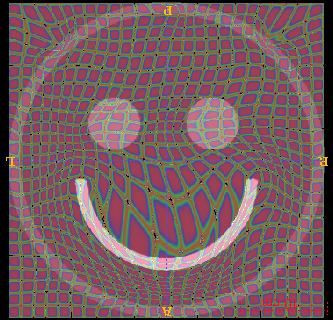
\includegraphics[width=0.45\textwidth]{Figures/frowntosmile.png}
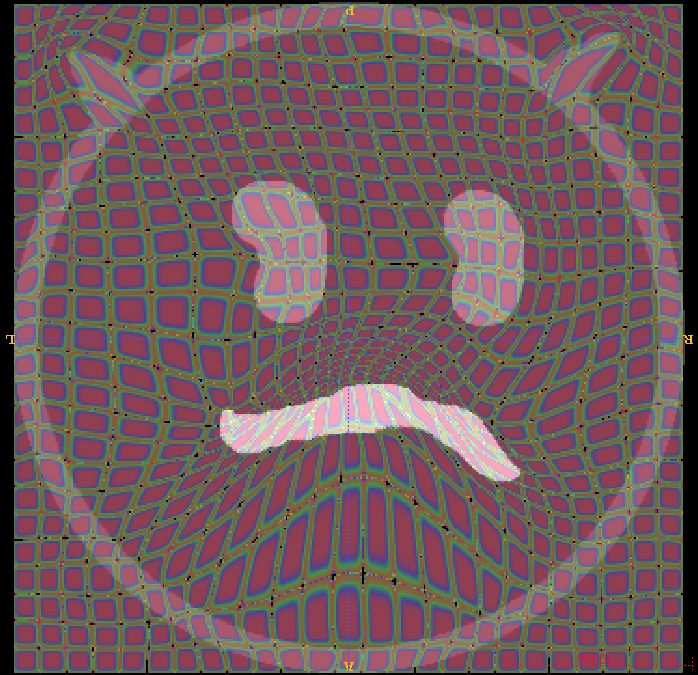
\includegraphics[width=0.45\textwidth]{Figures/smiletofrown.png}
\itkcaption[Frown To Smile]{Expected output for the frown to smile 
shows a smooth, though large deformation.  The grids are overlaid on 
the deformed images. }
\label{fig:frown}
\end{figure}
\begin{verbatim}
ANTs 2 -o PSEtest  -i 91x70x55x40x30  -r Gauss[3,0.] -t SyN[0.2]
   -m  PSE[Frown.nii,Smile.nii,Frown.nii,Smile.nii,0.75,0.1,11,0,10] 
   -m  MSQ[Frown.nii,Smile.nii,1,0]    --number-of-affine-iterations 0 

antsApplyTransforms  2 Frown.nii FrownToSmile.nii -R Smile.nii
   -i PSEtestAffine.txt PSEtestInverseWarp.nii 

antsApplyTransforms  2 Smile.nii SmileToFrown.nii -R Frown.nii 
    PSEtestWarp.nii PSEtestAffine.txt 

CreateWarpedGridImage 2 PSEtestInverseWarp.nii grid1.nii
CreateWarpedGridImage 2 PSEtestWarp.nii grid2.nii
\end{verbatim}
This example should run on the downloaded ANTs data so you may see the
results.
\end{comment}
%\input{ANTSLabeledDataExample}
%\input{ANTSMaskedImageRegistrationExample}



\newpage
\section{Data visualization with ANTs}
Data visualization is important for producing figures for manuscripts,
qualitative inspection of results, facilitating collaborations, and 
gaining insight into data and data transformations.  ANTs provides three
flexible programs to help with such tasks which we describe below.

\subsection{Creating faux-colormapped images with {\tt ConvertScalarImageToRGB}}
For layering image data, it is often useful to map the grayscale image intensity
values to distinct colormaps.  We introduced such a processing framework into
ITK described in \cite{Tustison2008c}.  The ANTs program {\tt ConvertScalarImageToRGB}
interfaces this framework and permits conversion of grayscale intensity scalar images
to RGB colormapped images which can be viewed in programs such as ITK-SNAP.  
Converting scalar images to RGB intensities is also a preprocessing step for 
the next two programs described:  {\tt CreateTiledMosaic} and {\tt antsSurf}.
In addition to the built-in colormaps which are currently part of ITK, we also 
have several custom colormaps located in the directory 
\verb#${ANTSPATH}/Examples/CustomColormaps/#.  Additionally, these custom colormaps
can be used as examples to build one's own set of colormaps for use with
{\tt ConvertScalarImageToRGB}. In Listing \ref{listing:ConvertScalarImageToRGB} we
give three code examples of converting grayscale intensity images to different 
colormaps with and without masks.

\lstset{frame = htb,
        framerule = 0.25pt,
        float,
        fontadjust,
        backgroundcolor={\color{listlightgray}},
        basicstyle = {\ttfamily\scriptsize},
        keywordstyle = {\ttfamily\color{listkeyword}\textbf},
        identifierstyle = {\ttfamily},
        commentstyle = {\ttfamily\color{listcomment}\textit},
        stringstyle = {\ttfamily},
        showstringspaces = false,
        showtabs = false,
        numbers = none,
        numbersep = 6pt,
        numberstyle={\ttfamily\color{listnumbers}},
        tabsize = 2,
        language=bash,
        floatplacement=!h,
        caption={\small Sample command calls to {\tt ConvertScalarImageToRGB} to produce different colormaps
        },
        captionpos=b,
        label=listing:ConvertScalarImageToRGB
        }
\begin{lstlisting}
# hot colormap
ConvertScalarImageToRGB 2 r16slice.nii.gz r16slice_hot.nii.gz none hot

# jet colormap (with a mask)
ThresholdImage 2 r16slice.nii.gz r16mask.nii.gz 0 0 0 1
ConvertScalarImageToRGB 2 r16slice.nii.gz r16slice_jet.nii.gz r16mask.nii.gz jet

# custom colormap (to show ITK-SNAP segmentation image)
ThresholdImage 2 r16slice.nii.gz r16mask.nii.gz 0 0 0 1
Atropos -d 2 -a r16slice.nii.gz -x r16mask.nii.gz -c [5,0] -i kmeans[3] -o r16seg.nii.gz
ConvertScalarImageToRGB 2 r16seg.nii.gz r16seg_snap.nii.gz \
  none custom ${ANTSPATH}/Examples/CustomColormaps/itkSnap.txt 0 6 0 255
\end{lstlisting}


\subsection{Figure production and large-scale data inspection using {\tt CreateTiledMosaic}}
The program {\tt CreateTiledMosaic} in conjunction with {\tt ConvertScalarImageToRGB} provides
useful functionality for common image analysis tasks.  The basic usage of {\tt CreateTiledMosaic}
is to tile a 3-D image volume slice-wise into a 2-D image.  The help menu {\tt CreateTiledMosaic --help}
provides more in-depth coverage of options but some of the functionality includes:
\begin{itemize}
  \item padding or cropping each tile element,
  \item alpha channel for translucent overlaid rob maps,
  \item flipping or permuting of each tile element, 
  \item comprehensive slice selection, and
  \item tiling pattern (i.e. custom number of rows and/or columns).
\end{itemize}

As a use case, suppose one wants
to quickly scroll through cortical thickness results from a processed cohort.  {\tt CreateTiledMosaic}
can be used to convert each processed subject into a 2-D .png image which can be easily scanned
for processing failures.  For example, in Listing \ref{listing:CreateTiledMosaic} we 
provide example code to process a subject {\tt OAS1\_0457\_MR1\_mpr\_n3\_anon\_sbj\_111} from the 
OASIS data set%
\footnote{
http://www.oasis-brains.org
}
after it has been processed by the {\tt antsCorticalThickness.sh} script.

\begin{figure}
\centering
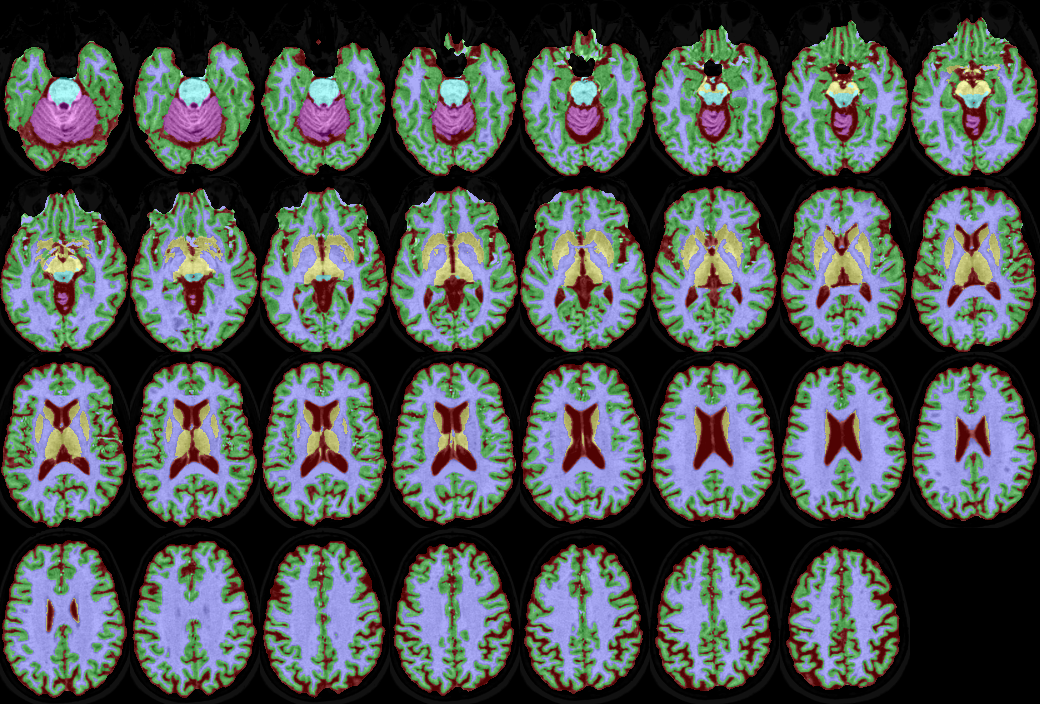
\includegraphics[width=0.8\textwidth]{Figures/OAS1_0457_MR1_mpr_n3_anon_sbj_111_segTiledMosaic.png}
\itkcaption[Tiled Mosaic]{Tiled mosaic showing every other axial slice of a single OASIS data 
subject with segmentation labels overlayed ($\alpha = 0.3$).
 }
\label{fig:oasis_seg}
\end{figure}

\begin{figure}
\centering
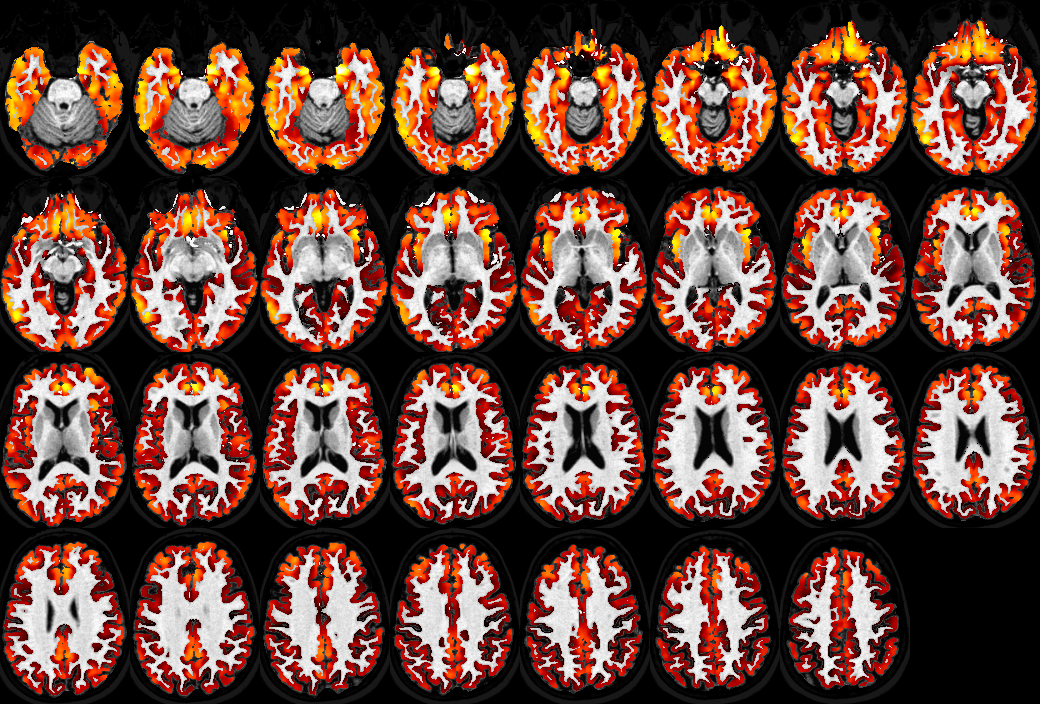
\includegraphics[width=0.8\textwidth]{Figures/OAS1_0457_MR1_mpr_n3_anon_sbj_111_tiledMosaic.png}
\itkcaption[Tiled Mosaic]{Tiled mosaic showing every other axial slice of a single OASIS data 
subject with thickness values overlayed in a ``hot'' colormap.
 }
\label{fig:oasis_thick}
\end{figure}


\lstset{frame = htb,
        framerule = 0.25pt,
        float,
        fontadjust,
        backgroundcolor={\color{listlightgray}},
        basicstyle = {\ttfamily\scriptsize},
        keywordstyle = {\ttfamily\color{listkeyword}\textbf},
        identifierstyle = {\ttfamily},
        commentstyle = {\ttfamily\color{listcomment}\textit},
        stringstyle = {\ttfamily},
        showstringspaces = false,
        showtabs = false,
        numbers = none,
        numbersep = 6pt,
        numberstyle={\ttfamily\color{listnumbers}},
        tabsize = 2,
        language=bash,
        floatplacement=!h,
        caption={\small Using {\tt CreateTiledMosaic} to visualize axial slices for 
        the OASIS data set subject {\tt OAS1\_0457\_MR1\_mpr\_n3\_anon\_sbj\_111}
        processed through the ANTs cortical thickness pipeline.
        },
        captionpos=b,
        label=listing:CreateTiledMosaic
        }
\begin{lstlisting}
##############################################################################
# Do segmentation mosaic
##############################################################################

itksnap=${ANTSPATH}/Examples/CustomColormaps/itkSnap.txt

# Convert segmentation labels to itk-snap label color scheme.  We set the min and max input 
# to [0,6] since we have only included the colors for labels 1-6 in the colormap.  If we 
# want to include more labels, we would need to modify the custom colormap.
ConvertScalarImageToRGB 3 OAS1_0457_MR1_mpr_n3_anon_sbj_111BrainSegmentation.nii.gz \
  OAS1_0457_MR1_mpr_n3_anon_sbj_111BrainSegmentation_snap.nii.gz none custom $itkSnap 0 6 0 255

# Create tiled segmentation mosaic.  We overlay "snap" segmentation map 
CreateTiledMosaic -i OAS1_0457_MR1_mpr_n3_anon_sbj_111BrainSegmentation0N4.nii.gz \
  -r OAS1_0457_MR1_mpr_n3_anon_sbj_111BrainSegmentation_snap.nii.gz \
  -o OAS1_0457_MR1_mpr_n3_anon_sbj_111_tiledMosaic.png \
  -a 0.3 -t -1x8 -d 2 -p [-15x-50,-15x-30,0] -s [2,100,160]

##############################################################################
# Do thickness mosaic
##############################################################################

# Convert thickness map to hot color map.  We scale thickness values
#  between [0,8] to the standard RGB range of [0,255]
ConvertScalarImageToRGB 3 OAS1_0457_MR1_mpr_n3_anon_sbj_111CorticalThickness.nii.gz \
  OAS1_0457_MR1_mpr_n3_anon_sbj_111CorticalThickness_hot.nii.gz none hot none 0 8 0 255

# Create a mask for next call
ThresholdImage 3 OAS1_0457_MR1_mpr_n3_anon_sbj_111CorticalThickness.nii.gz \
  OAS1_0457_MR1_mpr_n3_anon_sbj_111CorticalThickness_mask.nii.gz 0 0 0 1

# Create tiled mosaic.  We overlay "hot" thickness map (but only the values within
# the mask on the bias corrected structural MR image
CreateTiledMosaic -i OAS1_0457_MR1_mpr_n3_anon_sbj_111BrainSegmentation0N4.nii.gz \
  -r OAS1_0457_MR1_mpr_n3_anon_sbj_111CorticalThickness_hot.nii.gz \
  -x OAS1_0457_MR1_mpr_n3_anon_sbj_111CorticalThickness_mask.nii.gz \
  -o OAS1_0457_MR1_mpr_n3_anon_sbj_111_tiledMosaic.png \
  -a 1.0 -t -1x8 -d 2 -p [-15x-50,-15x-30,0] -s [2,100,160]
\end{lstlisting}


\subsection{Volumetric visualizations with {\tt antsSurf}}
Our third program, {\tt antsSurf}, is used to produce volumetric surface
renderings from binary images with optional functional overlays.  Again,
the {\tt antsSurf} help menu provides a more comprehensive description of
functionality but some available options include:
\begin{itemize}
  \item specification of more than one functional overlay,
  \item painting of functional overlays based on order on the command line,
  \item localization of the functional overlay within a specified masked region,
  \item manual reorientation,
  \item manual adjustment of solid background and surface colors, and
  \item simple estimation of binary image given a mesh.
\end{itemize}
Reverting back to our OASIS cortical thickness example, we render three surfaces
using {\tt antsSurf} in Figure \ref{fig:oasis_gm_wm} which demonstrate some of 
the main capabilities of {\tt antsSurf} and how one would incorporate other
ANTs tools.  The code to produce Figure \ref{fig:oasis_gm_wm} is located in 
Listing \ref{listing:antsSurf}.

\lstset{frame = htb,
        framerule = 0.25pt,
        float,
        fontadjust,
        backgroundcolor={\color{listlightgray}},
        basicstyle = {\ttfamily\scriptsize},
        keywordstyle = {\ttfamily\color{listkeyword}\textbf},
        identifierstyle = {\ttfamily},
        commentstyle = {\ttfamily\color{listcomment}\textit},
        stringstyle = {\ttfamily},
        showstringspaces = false,
        showtabs = false,
        numbers = none,
        numbersep = 6pt,
        numberstyle={\ttfamily\color{listnumbers}},
        tabsize = 2,
        language=bash,
        floatplacement=!h,
        caption={\small Using {\tt antsSurf} to visualize volumes associated with
        the OASIS data set subject {\tt OAS1\_0457\_MR1\_mpr\_n3\_anon\_sbj\_111}
        processed through the ANTs cortical thickness pipeline.
        },
        captionpos=b,
        label=listing:antsSurf
        }
\begin{lstlisting}
##############################################################################
# Do a simple volume rendering of the gray and white matters
##############################################################################

# Create gray matter binary image
ThresholdImage 3 OAS1_0457_MR1_mpr_n3_anon_sbj_111BrainSegmentation.nii.gz \
  OAS1_0457_MR1_mpr_n3_anon_sbj_111BrainSegmentationGm.nii.gz 2 2 1 0

# Volumetrically render the gray matter using a terrible color choice and reorient
antsSurf -s [OAS1_0457_MR1_mpr_n3_anon_sbj_111BrainSegmentationGm.nii.gz,255x0x255] \
  -d OAS1_0457_MR1_mpr_n3_anon_sbj_111GrayMatter.png[90x180x90,255x128x0]

# Create white matter binary image
ThresholdImage 3 OAS1_0457_MR1_mpr_n3_anon_sbj_111BrainSegmentation.nii.gz \
  OAS1_0457_MR1_mpr_n3_anon_sbj_111BrainSegmentationWm.nii.gz 3 3 1 0

# Volumetrically render the white matter using a terrible color choice and reorient
antsSurf -s [OAS1_0457_MR1_mpr_n3_anon_sbj_111BrainSegmentationWm.nii.gz,139x69x19] \
  -d  OAS1_0457_MR1_mpr_n3_anon_sbj_111WhiteMatter.png[90x180x90,178x34x34]

##############################################################################
# Render the cortical thickness map on the gray matter surface
##############################################################################

# dilate the cortical thickness values to ensure values cover the entire GM surface
ImageMath 3 OAS1_0457_MR1_mpr_n3_anon_sbj_111CorticalThicknessDilated.nii.gz GD \
  OAS1_0457_MR1_mpr_n3_anon_sbj_111CorticalThickness.nii.gz 1

# create a corresponding mask
ThresholdImage 3 OAS1_0457_MR1_mpr_n3_anon_sbj_111CorticalThicknessDilated.nii.gz \
  OAS1_0457_MR1_mpr_n3_anon_sbj_111CorticalThicknessDilated_mask.nii.gz 0 0 0 1

# convert to hot color map
ConvertScalarImageToRGB 3 OAS1_0457_MR1_mpr_n3_anon_sbj_111CorticalThicknessDilated.nii.gz \
  OAS1_0457_MR1_mpr_n3_anon_sbj_111CorticalThicknessDilated_hot.nii.gz none hot none 0 8 0 255
  
# Render the gray matter with superimposed cortical thickness values
antsSurf -s OAS1_0457_MR1_mpr_n3_anon_sbj_111BrainSegmentationGm.nii.gz \
  -f [OAS1_0457_MR1_mpr_n3_anon_sbj_111CorticalThicknessDilated_hot.nii.gz, \
      OAS1_0457_MR1_mpr_n3_anon_sbj_111CorticalThicknessDilated_mask.nii.gz] \
  -d  OAS1_0457_MR1_mpr_n3_anon_sbj_111CorticalThickness.png[90x180x90]
\end{lstlisting}  

\begin{figure}
\centering
\begin{tabular}{ccc}
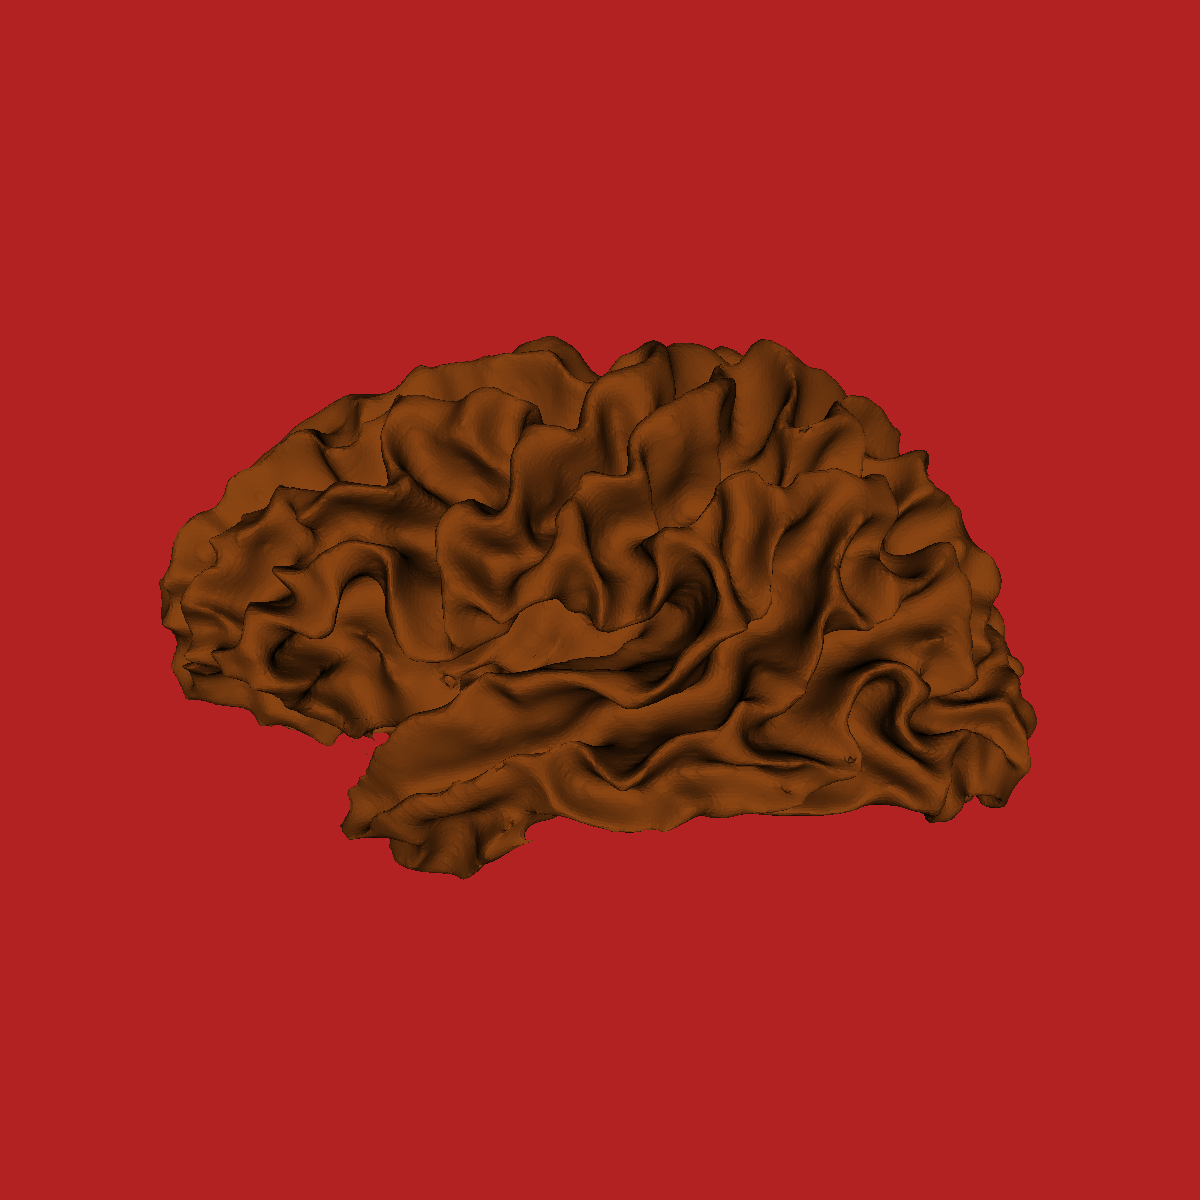
\includegraphics[width=0.315\textwidth]{Figures/OAS1_0457_MR1_mpr_n3_anon_sbj_111WhiteMatter.png} &
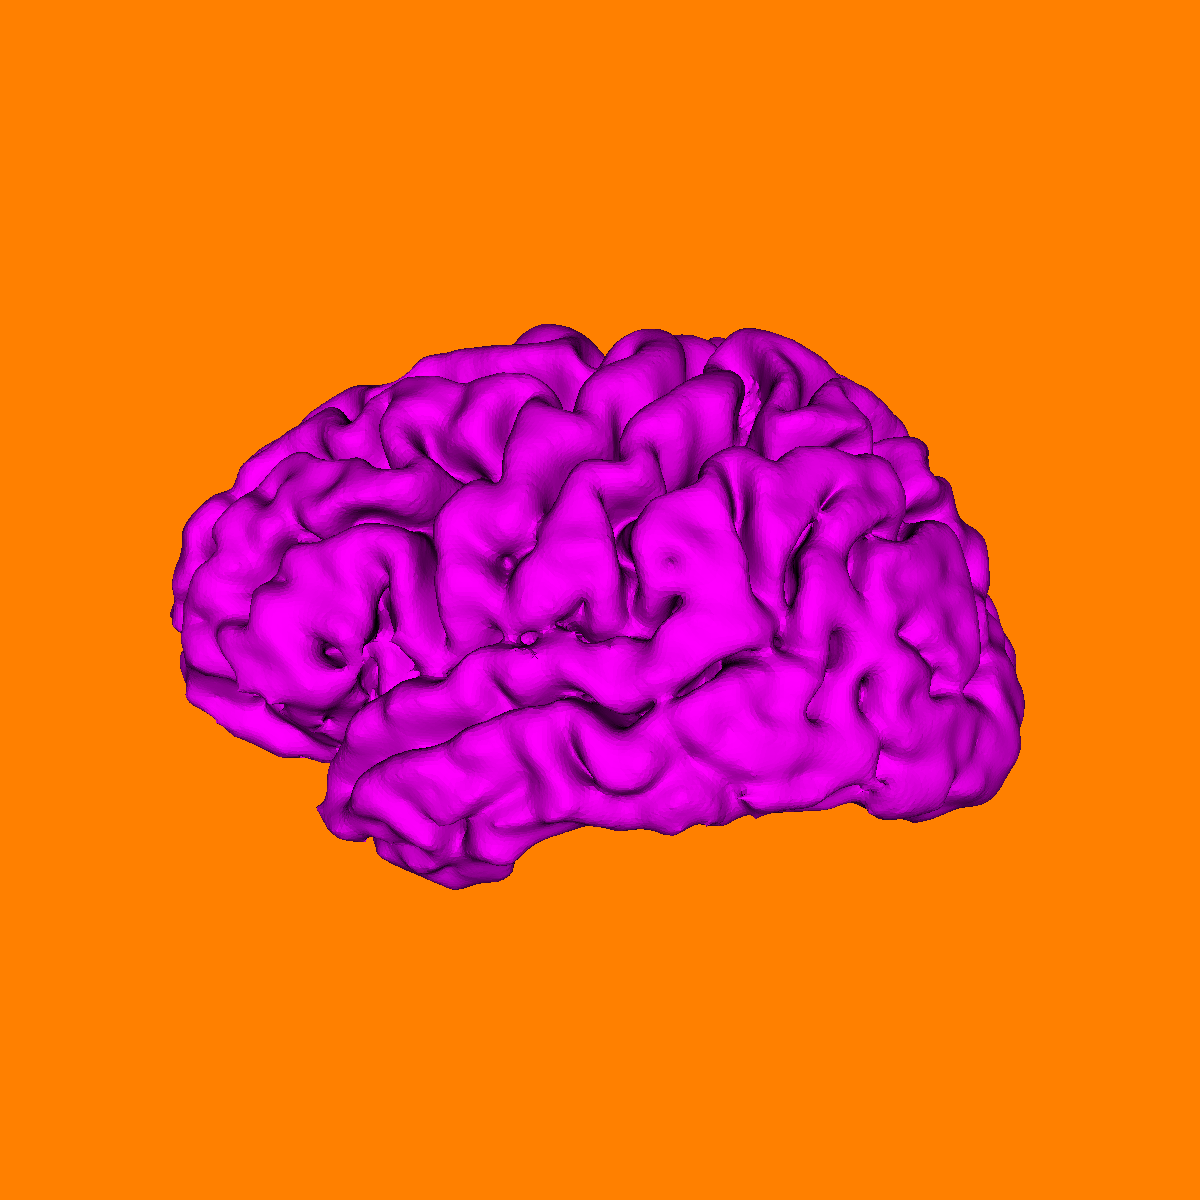
\includegraphics[width=0.315\textwidth]{Figures/OAS1_0457_MR1_mpr_n3_anon_sbj_111GrayMatter.png} &
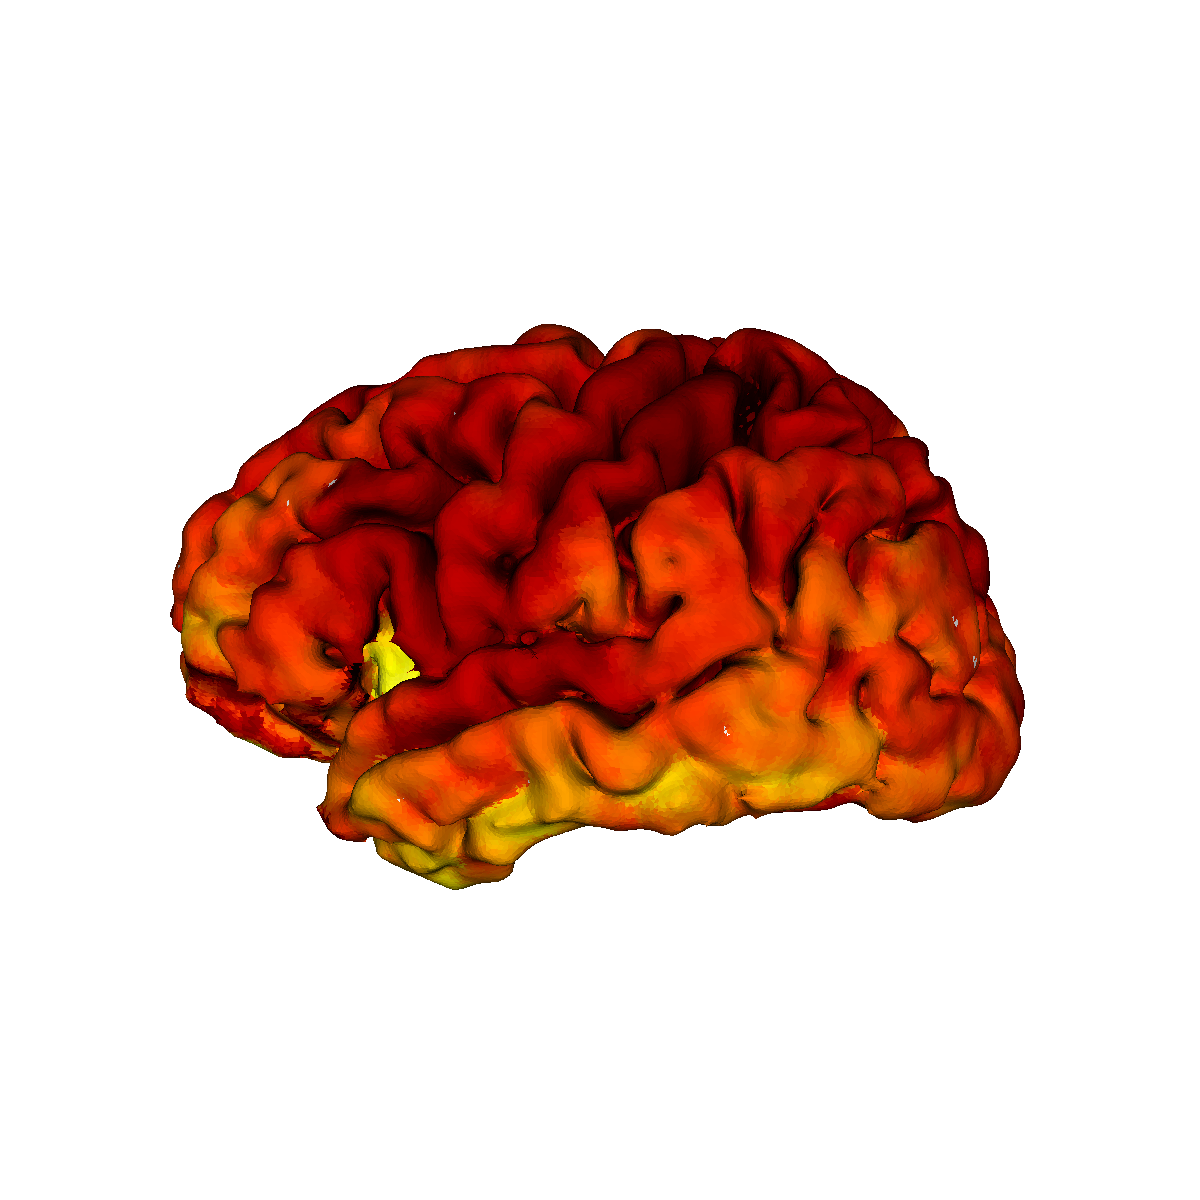
\includegraphics[width=0.315\textwidth]{Figures/OAS1_0457_MR1_mpr_n3_anon_sbj_111CorticalThickness.png} \\
white matter & gray matter & cortical thickness
\end{tabular}
\itkcaption[Volumetric rendering with antsSurf]{Volumetric renderings of {\tt OAS1\_0457\_MR1\_mpr\_n3\_anon\_sbj\_111} data set using {\tt antsSurf}.}
\label{fig:oasis_gm_wm}
\end{figure}



\newpage \newpage
\section{ANTs-based studies}
We've performed several types of applied studies with ANTs.  Some of
my favorite include our recent work on eigenanatomy
\href{http://scholar.google.com/scholar?q=eigenanatomy+avants&btnG=&hl=en&as_sdt=0%2C39}{eigenanatomy-gs},
\href{http://www.ncbi.nlm.nih.gov/pubmed/?term=eigenanatomy}{eigenanatomy-pubmed}
and sccan \href{http://scholar.google.com/scholar?q=canonical+correlation+avants&btnG=&hl=en&as_sdt=0%2C39}{sccan-gs},
\href{http://www.ncbi.nlm.nih.gov/pubmed/?term=canonical+correlation+avants}{sccan-pubmed} 
\href{}{} as well as a recent large-scale comparison with Freesurfer (if interested,
google it).  These all use open source tools that are freely available
via ANTs and/or \textit{ANTsR}.  We are also currently validating significant
resources for processing BOLD and ASL functional MRI.

\subsection{Brain mapping in the presence of lesions}
Many cases violate the basic assumption of a one-to-one mapping from a
template image to a target image. Brain lesions caused by stroke or
traumatic brain injury are a common instance of this.

The ANTs toolkit handles this situation by a constrained cost-function
masking approach. In short, the mapping within an excluded region (as
determined by an inclusive mask) is determined by the solution outside
of the region. To achieve this with ANTs, one would use a call similar
to this \href{http://stnava.github.io/BasicBrainMapping/}{http://stnava.github.io/BasicBrainMapping/}.
The additional parameter needed for this approach 
is the \texttt{-x}  \texttt{mask.nii.gz}  which 
is the mask defined in the ``fixed" (or individual) image space.  
Mask values above 0.5 are considered non-outlier or non-lesioned regions.
The labeling may be performed with ITK-SNAP. 
Figure~\ref{fig:lesion} illustrates the approach.
\begin{figure}
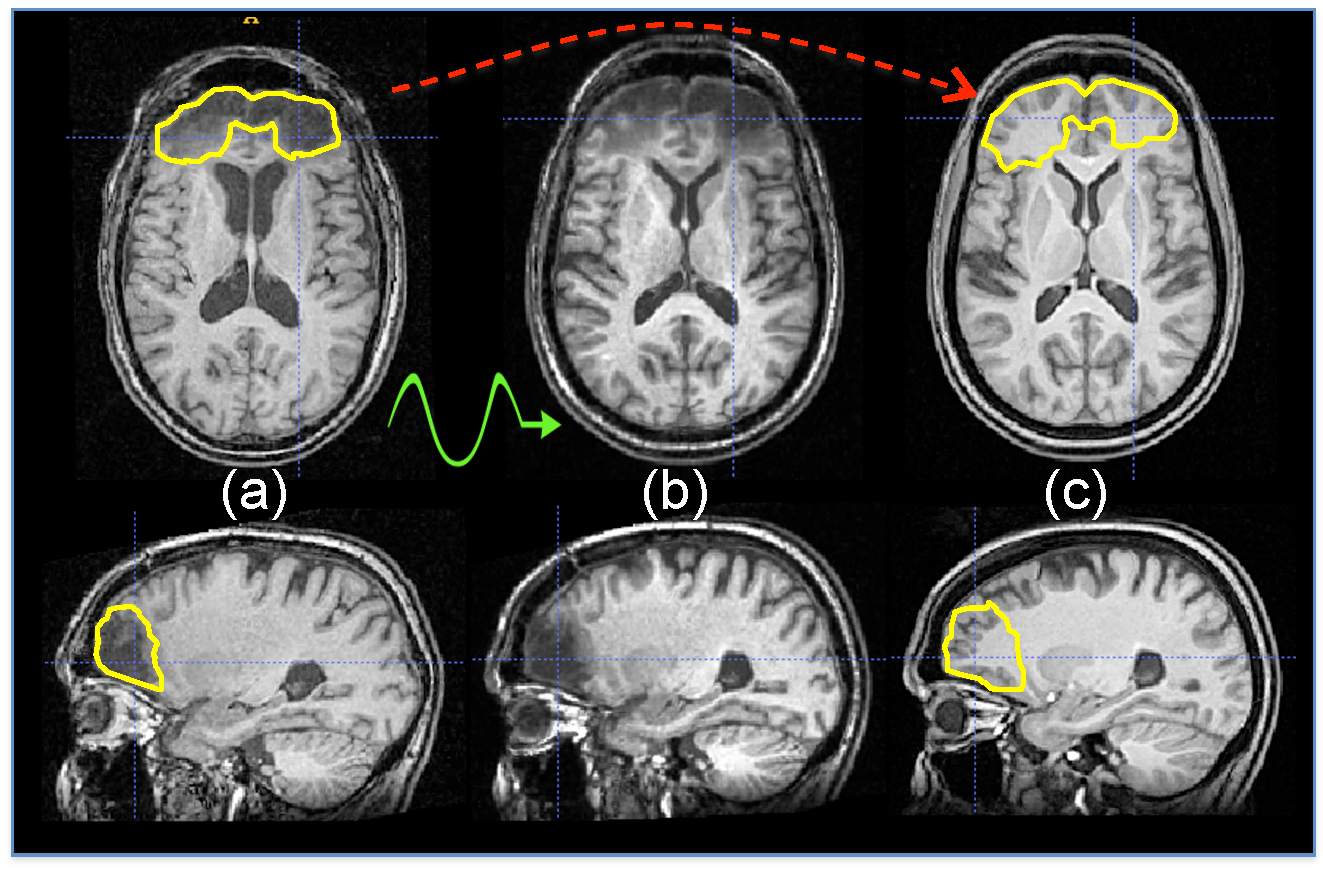
\includegraphics[width=1\textwidth]{Figures/lesionstudy.pdf}
\itkcaption[ANTs Lesions]{Here, we see a semi-automated approach for lesion analysis
based on diffeomorphic normalization.  The user outlines the lesion
site in the subject space, as shown in (a).  Diffeomorphic mapping is
then used to deform the subject image in (a) into the space of the
reference template.  The deformed subject is shown in panel (b).
Panel (c) shows the reference template space with the estimated
position of the subject's lesion overlaid on the healthy tissue of the
template.  This approach enables one to compare the subject image
against prior information stored in the template space such as
anatomical labels or statistics on the appearance of lesioned and/or
normal tissue.}
\label{fig:lesion}
\end{figure}
Once the ANTs mapping is solved, 
one is able to estimate the location of the lesion in the template space by mapping the inverse lesion mask to the template.
To take the negative image of the inclusive mask 
and warp the mask to the template :
\begin{verbatim}
ImageMath 3 lesionmask.nii.gz Neg inclusivemask.nii.gz
antsApplyTransforms -d 3 -i lesionmask.nii.gz -o lesiontotemplate.nii.gz 
   -r template.nii.gz -t [output0GenericAffine.mat,1] -t output1InverseWarp.nii.gz
\end{verbatim}
There are several examples of this approach in the literature:
\href{http://www.ncbi.nlm.nih.gov/pubmed/?term=coslett+kim+injury}{http://www.ncbi.nlm.nih.gov/pubmed/?term=coslett+kim+injury}
or
\href{http://scholar.google.com/scholar?q=brain+normalization+MRI+ANTs+advanced+lesion+tools+-ant&btnG=&hl=en&as_sdt=0%2C39}{relevant google-scholar search}.
See also: \href{http://www.ncrrn.org/papers/methodology\_papers/sp\_norm\_kim.pdf}{http://www.ncrrn.org/papers/methodology\_papers/sp\_norm\_kim.pdf}.

\subsection{Statistical mapping with ANTs: Morphometry, function, jacobian, thickness}
ANTs has been applied in a wide array of imaging studies
\cite{Avants2009a,Avants2009b,Avants2009,Das2009,Klein2009,Massimo2009,Pluta2008,Tustison2009,Yushkevich2009,Avants2008c,Avants2008b,M.Grossman10282008,Kim2008,Simon2008,Sun2008,Yushkevich2008,Aguirre2007,Avants2007,Avants2007i}.
All of these studies benefit in some way from normalization whether the topic is cortical
thickness, Jacobian-based morphometry, volumetric morphometry or functional studies. 
From a broad perspective, each of these applications requires the same steps:
\begin{enumerate}
\item Preprocess images -- bias correction, segmentation, etc.  Potentially construct an optimal template. 
\item Normalize images -- run \texttt{antsRegistrationSyN.sh} to map a population of images to a template and store the deformations. 
\item Derive any data from the deformation that may be necessary, e.g. the log-Jacobian.
\item Apply the warp to any images one may want to analyze in template space.  
\item Perform statistics in template space over the region of interest, e.g. all cortex. 
\end{enumerate}
We now list ANTs tools needed for basic morphometry and/or brain labeling.
Typical output is in figure~\ref{fig:morph}.
\begin{verbatim}
0.  antsMultivariateTemplateConstruction2.sh for template building
1.  antsRegistration
2.  antsApplyTransforms for mapping between spaces
3.  Atropos for segmentation.
4.  SmoothImage for smoothing  
5.  CreateJacobianDeterminantImage for computing the jacobian
6.  antsMalfLabeling.sh | jointfusion for convenient multi-template labeling
\end{verbatim}
See \cite{Wang2011} to learn more about joint fusion.
\begin{figure}
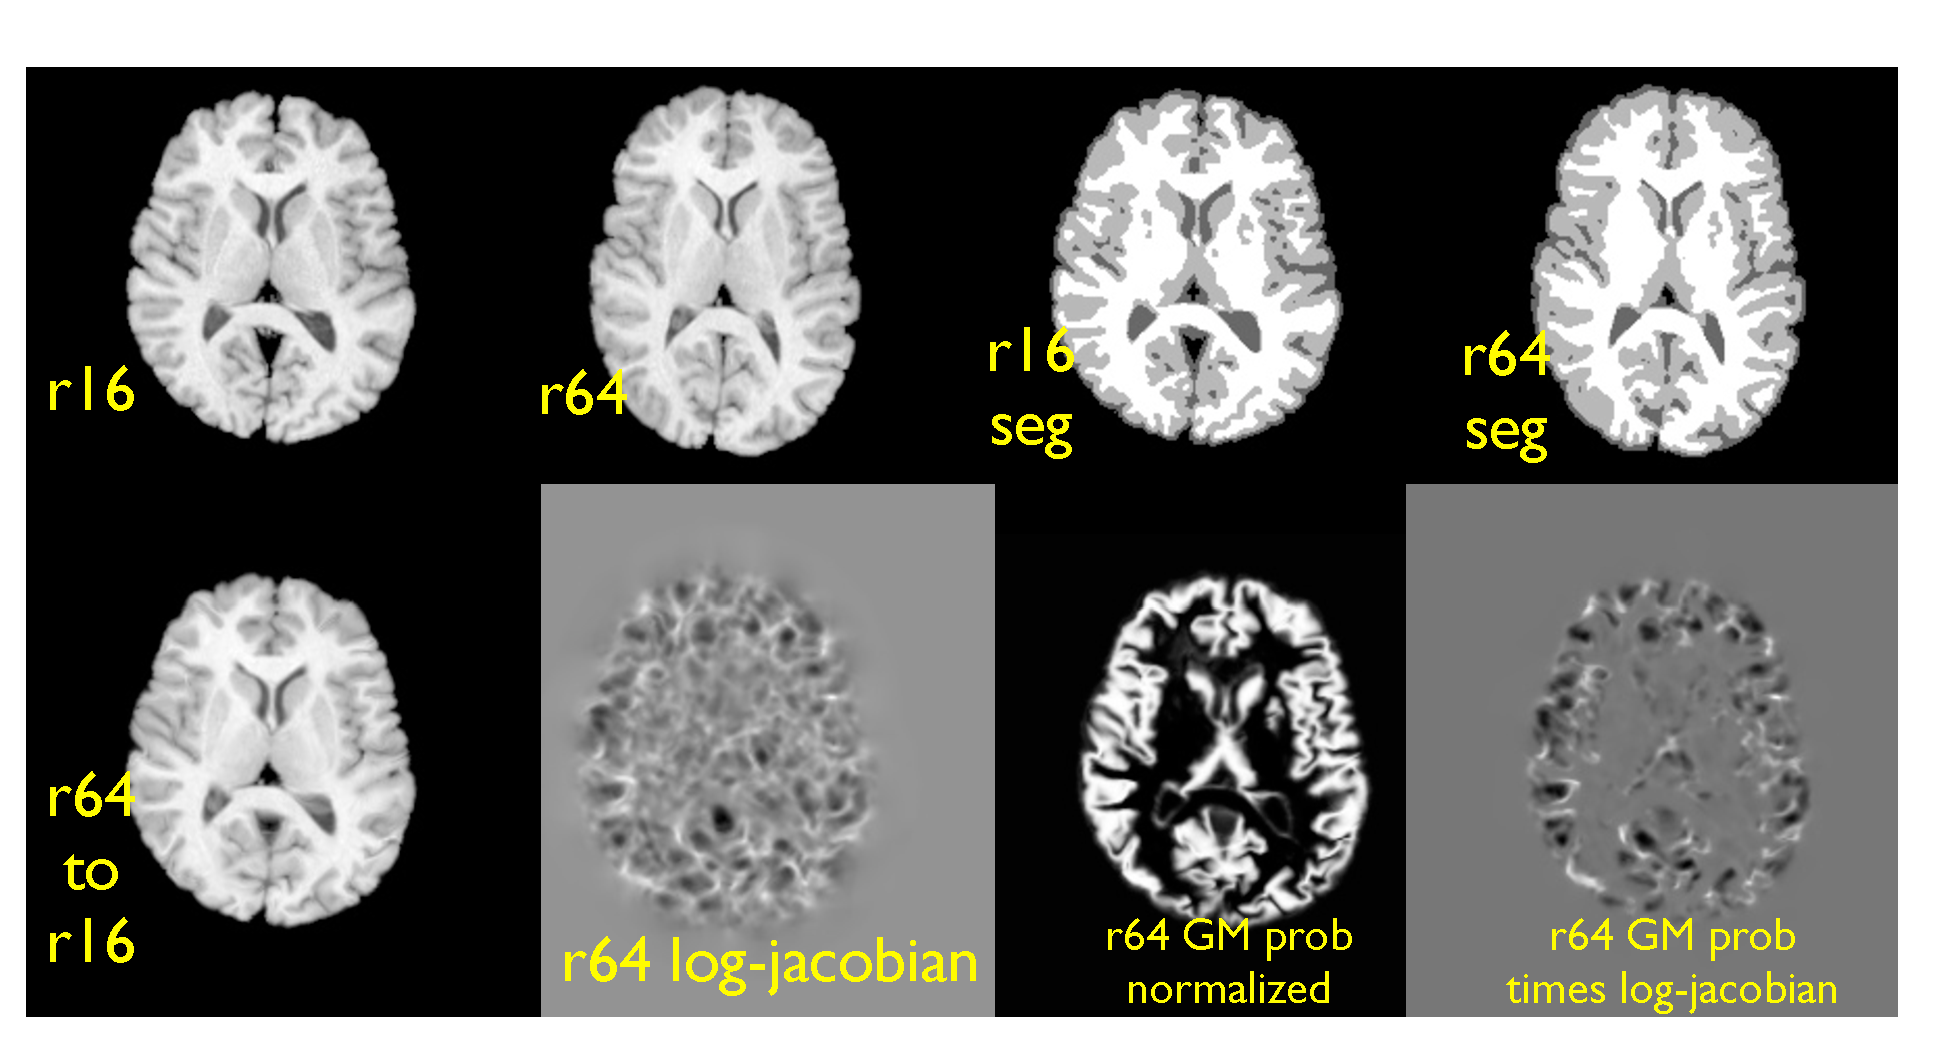
\includegraphics[width=1\textwidth]{Figures/morphometry.pdf}
\itkcaption[ANTs Morphometry]{The output from the ANTs morphometry example.}
\label{fig:morph}
\end{figure}
Figure~\ref{fig:morph} shows a more or less standard Jacobian-based approach to morphometry.
Often, we use the log-Jacobian because it is symmetric about zero.
Some suggest to mask with the gray matter segmentation to restrict the analysis to the
cortex.  The Jacobian is discussed in figure~\ref{fig:inv} and visualization of
the Jacobian is shown in figure~\ref{fig:jac}.  This Jacobian comes
from the mapping shown in figure~\ref{fig:large}.
\begin{figure}
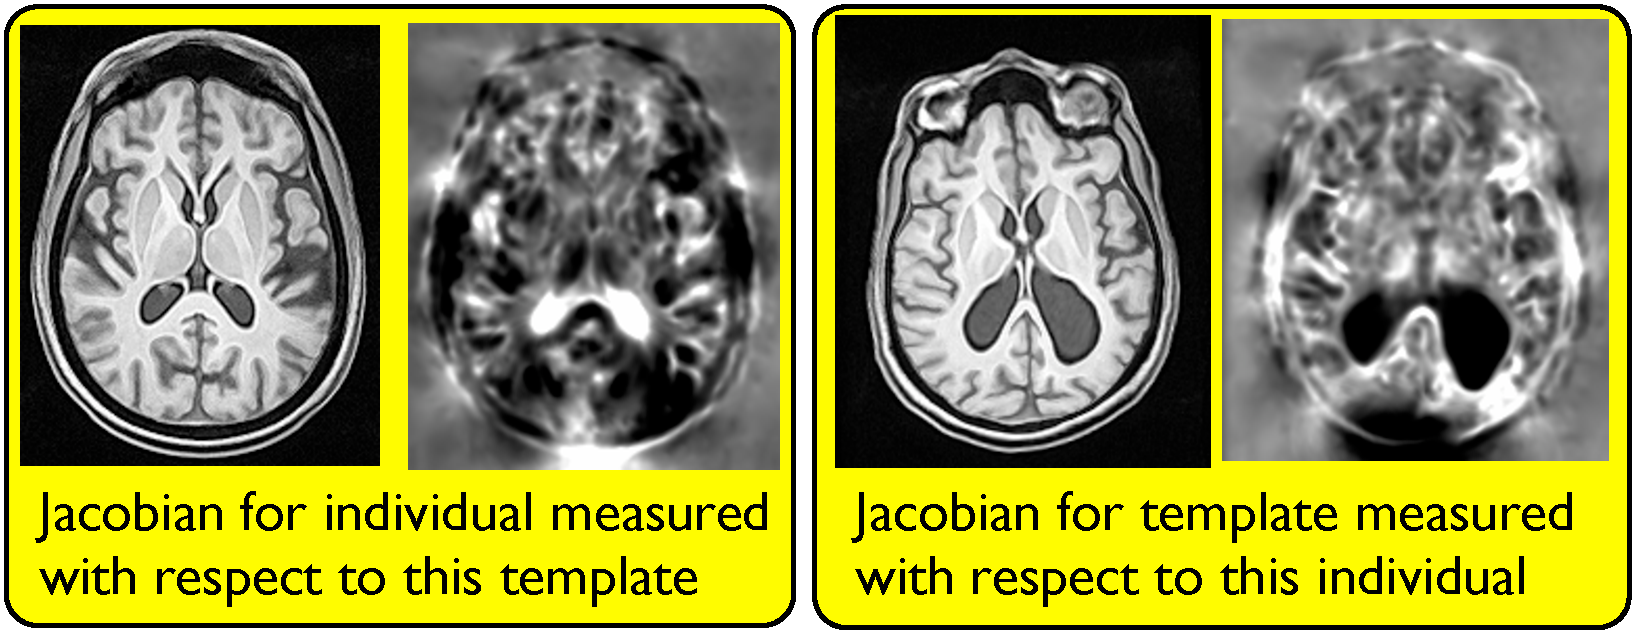
\includegraphics[width=1\textwidth]{Figures/Jacobian.pdf}
\itkcaption[ANTs Jacobian]{The Jacobian: Note that the bright values
  in the template image ventricles (left) indicate that the ventricles
  are relatively larger in the subject image. Similarly, the dark
  jacobian values in the individual image show that the template has
  smaller ventricles. This example is described on the large
  deformation page Large Def. Once one gains the Jacobian (or more
  appropriately, the log-Jacobian), then one may compute statistics
  across the population.}
\label{fig:jac}
\end{figure}
Many analyses may be performed on data that may be derived using ANTs:
thickness images, functional images or fractional anisotropy images derived from the diffusion 
tensor modality.  In all these cases, the tools listed above and
throughout this document should be very helpful.

\subsection{Statistics with ANTs and \texttt{R}: \texttt{ANTsR} }
\texttt{R} is an open-source, cutting-edge statistical package 
used by statisticians world-wide.   ANTs is designed to 
interface with \texttt{R} via the \texttt{ANTsR} package.  Google
this and learn more. Most statistical requirements may be met with this setup. 
\newpage
\section{Dependencies and Related Software}

\subsection{How to build ANTs/ANTsR for users who are new to
  scientific computing}\label{sec:comp0}
We maintain an installation script for OSX and LINUX variants that
attempts to automate installation of the build environment you need
for ANTs and many other scientific computing resources.  The script is
here:
\href{https://raw.githubusercontent.com/stnava/RMI/master/stnava/install_anstr_packages.sh}{ANTs
install script (link)}.  You can run the script directly but you
might, instead, want to follow the steps one by one so you learn a
little bit about what it does.  At the end of the script, ANTs and its
binaries and scripts (the ANTs/Scripts directory) should be installed
within a subdirectory of the ANTsR source tree.

\subsection{Dependencies and Compilation}\label{sec:comp}
If you already have a build environment set up on your computer, these 
instructions should work for you.
ANTs depends on the most recent version of the Insight ToolKit (ITK)
-- www.itk.org.  However, there is no need to download ITK separately.
ANTs and ITK are both compiled through CMake which automates the
process.  We describe this here: 
\begin{verbatim}
instructions for linux / osx type installation.   
windows works too ( via cmake ) but i dont have specifics.

to compile ants from the source code, you first need: git, cmake and a c++ compiler

then in a terminal, do:

>  git clone git://github.com/stnava/ANTs.git
>  mkdir antsbin

> cd antsbin

>  ccmake ../ANTs

then go into cmake and type “c” and then “g”  then exit back to the
terminal.   then:

>  make -j 1

and wait a while.  you can change 1 to n-cores if you're feeling lucky.

to update an existing ANTs install, go to the ANTs directory and type 

“git pull origin master”

Don’t forget to toggle to advanced and turn off

SuperBuild_ANTS_USE_GIT_PROTOC if behind firewall
\end{verbatim}
We (used to) maintain a dashboard to give users an idea of what to expect 
from compilation:\newline
\href{http://testing.psychiatry.uiowa.edu/CDash/index.php?project=ANTS}{ANTs
Dashboard: http://testing.psychiatry.uiowa.edu/CDash/index.php?project=ANTS}
\textcolor{red}{Needs to be rebooted pending funding/space etc.}

\subsection{Visualization and Quantification of ANTs Results}
Use \href{www.itksnap.org}{itk SNAP : www.itksnap.org } or mricro / mricron for viewing
images.  The ANTs program StackSlices can be used to conveniently scan
through a dataset in any of its axes.  It is useful for checking both
input data quality and output normalization quality.  MeasureImageSimilarity 
will supply numerical measures of image similarity via three different metrics. 

\subsection{Pipelining with ANTs}
Use PipeDream for automating large-scale processing:\newline
\href{https://github.com/cookpa/pipedream}{PipeDream
  Homepage :
  https://github.com/cookpa/pipedream} \newline PipeDream
is integrated with ANTs and automates more complex studies such as
multivariate diffusion tensor and T1 cortical thickness studies,
longitudinal mapping and reconstruction of nifti images from Dicom.
\newpage
\section{Annotated Bibliography (Old)}
The original statement of the symmetric normalization and template
construction methodology was given in \cite{Avants2004} with a more 
recent template paper here \cite{Avants2009c}. 
A follow up study that used landmark guidance to compare the chimpanzee cortex to
the human cortex was published here \cite{Avants2006} -- this study
used {\em in vivo} MRI and template-based normalization to confirm
volumetric numbers derived from an early 20th century post-mortem
study comparing one human and one chimp.  This conference article has
some additional detail and alternative updates to the methodology, in
particular application to shape-based interpolation
\cite{Avants2005b}.  Network based studies were performed here
\cite{duda08miccai,duda08cvpr}.  The main SyN paper is here
\cite{Avants2008}.  Applications to neurodegeration are here
\cite{Avants2005,Avants2008a,Grossman2008,Avants2009,Das2009,Yushkevich2009,Massimo2009}.
Hippocampus focused work is here \cite{Pluta2009,Yushkevich2009}.  The
main evaluation papers include \cite{Avants2008} and \cite{Klein2009}
for the cortex and deep brain structures whereas \cite{Pluta2009}
evaluates the use of automated and semi-automated normalization for
high-throughput hippocampus morphometry.  An additional evaluation
paper is being developed.  


%%%%%%%%%%%%%%%%%%%%%%%%%%%%%%%%%%%%%%%%%
%
%  Insert the bibliography using BibTeX
%
%%%%%%%%%%%%%%%%%%%%%%%%%%%%%%%%%%%%%%%%%

\bibliographystyle{plain}
\bibliography{ants,references}


\end{document}

